\documentclass[
11pt, % The default document font size, options: 10pt, 11pt, 12pt
%oneside, % Two side (alternating margins) for binding by default, uncomment to switch to one side
english, % ngerman for German
singlespacing, % Single line spacing, alternatives: onehalfspacing or doublespacing
%draft, % Uncomment to enable draft mode (no pictures, no links, overfull hboxes indicated)
%nolistspacing, % If the document is onehalfspacing or doublespacing, uncomment this to set spacing in lists to single
%liststotoc, % Uncomment to add the list of figures/tables/etc to the table of contents
%toctotoc, % Uncomment to add the main table of contents to the table of contents
%parskip, % Uncomment to add space between paragraphs
%nohyperref, % Uncomment to not load the hyperref package
headsepline, % Uncomment to get a line under the header
%chapterinoneline, % Uncomment to place the chapter title next to the number on one line
%consistentlayout, % Uncomment to change the layout of the declaration, abstract and acknowledgements pages to match the default layout
]{MastersDoctoralThesis} % The class file specifying the document structure

\usepackage[utf8]{inputenc} % Required for inputting international characters
\usepackage[T1]{fontenc} % Output font encoding for international characters

\usepackage{datetime}

\newcommand\hmmax{0}
\newcommand\bmmax{0}

\newdateformat{monthyeardate}{%
  \monthname[\THEMONTH], \THEYEAR}

\usepackage{mathpazo} % Use the Palatino font by default

\usepackage[backend=bibtex,style=ieee,natbib=true]{biblatex}

\usepackage{amsmath,amssymb,amsfonts,bm}
\usepackage{scalerel}
\usepackage{mathtools}
\usepackage{graphicx}
\usepackage{float}
\usepackage{mathrsfs}
\usepackage{hyperref}
\usepackage{subcaption}
\usepackage{graphicx}
\usepackage{textcomp}
\usepackage{booktabs}
\usepackage{pifont}
\usepackage{enumitem}
\usepackage{xcolor}

% Bright noticeable placeholders for missing/TODO 
\newcommand{\citeplaceholder}[1]{\textbf{[Cite #1]}}
\newcommand{\placeholderfigure}[1][width=0.8\textwidth]{\fbox{\parbox{#1}{\centering Placeholder for Figure}}}
\newcommand{\placeholdertext}[1]{\textcolor{red}{\textbf{[PLACEHOLDER: #1]}}}

\addbibresource{refs.bib} % The filename of the bibliography

\usepackage[autostyle=true]{csquotes} % Required to generate language-dependent quotes in the bibliography

%----------------------------------------------------------------------------------------
%	MARGIN SETTINGS
%----------------------------------------------------------------------------------------

\geometry{
	paper=a4paper, % Change to letterpaper for US letter
	inner=2.5cm, % Inner margin
	outer=3.8cm, % Outer margin
	bindingoffset=.5cm, % Binding offset
	top=1.5cm, % Top margin
	bottom=1.5cm, % Bottom margin
	%showframe, % Uncomment to show how the type block is set on the page
}

%----------------------------------------------------------------------------------------
%	THESIS INFORMATION
%----------------------------------------------------------------------------------------

\thesistitle{From Sparse Records to Spatial Insights: Clustering and GIS Techniques in Analysis of Named Erratics} % Your thesis title, this is used in the title and abstract, print it elsewhere with \ttitle

\supervisor{Prof. Mahdi \textsc{Agheli}\\Prof. Guanrui \textsc{Li}} % Your supervisor's name, this is used in the title page, print it elsewhere with \supname

\examiner{} % Your examiner's name, this is not currently used anywhere in the template, print it elsewhere with \examname

\degree{Bachelor of Science} % Your degree name, this is used in the title page and abstract, print it elsewhere with \degreename

\author{Ethan \textsc{Chandler}} % Your name, this is used in the title page and abstract, print it elsewhere with \authorname

\addresses{} % Your address, this is not currently used anywhere in the template, print it elsewhere with \addressname

\subject{} % Your subject area, this is not currently used anywhere in the template, print it elsewhere with \subjectname

\keywords{} % Keywords for your thesis, this is not currently used anywhere in the template, print it elsewhere with \keywordnames

\university{\href{https://www.wpi.edu/}{Worcester Polytechnic Institute}} % Your university's name and URL, this is used in the title page and abstract, print it elsewhere with \univname

\department{} % Your department's name and URL, this is used in the title page and abstract, print it elsewhere with \deptname

\group{\href{https://www.wpi.edu/}{Worcester Polytechnic Institute}} % Your research group's name and URL, this is used in the title page, print it elsewhere with \groupname

\faculty{} % Your faculty's name and URL, this is used in the title page and abstract, print it elsewhere with \facname

\AtBeginDocument{
\hypersetup{pdftitle=\ttitle} % Set the PDF's title to your title
\hypersetup{pdfauthor=\authorname} % Set the PDF's author to your name
\hypersetup{pdfkeywords=\keywordnames} % Set the PDF's keywords to your keywords
}

\begin{document}

\frontmatter % Use roman page numbering style (i, ii, iii, iv...) for the pre-content pages

\pagestyle{plain} % Default to the plain heading style until the thesis style is called for the body content

%----------------------------------------------------------------------------------------
%	TITLE PAGE
%----------------------------------------------------------------------------------------

\begin{titlepage}
\begin{center}

% \vspace*{.06\textheight}
\vspace*{1px}
{\scshape\LARGE \univname\par}\vspace{1.5cm} % University name
\textsc{\Large Interactive Qualifying Project}\\[0.5cm] % Thesis type

\HRule \\[0.4cm] % Horizontal line
{\huge \bfseries \ttitle\par}\vspace{0.4cm} % Thesis title
\HRule \\[1.5cm] % Horizontal line
 
\begin{minipage}[t]{0.4\textwidth}
\begin{flushleft} \large
\emph{Author:}\\
\href{https://www.linkedin.com/in/echandler5956f/}{\authorname}\\ % Author name - remove the \href bracket to remove the link
\vspace{0.4cm}
\emph{Supervisor:} \\
\href{https://www.wpi.edu/people/faculty/jcocola}{Professor Jim \textsc{Cocola}}\\
{\small \bfseries Worcester Polytechnic Institute}
\end{flushleft}
\end{minipage}
\begin{minipage}[t]{0.4\textwidth}
\begin{flushright} \large
% \emph{Supervisor:} \\
% \href{https://www.wpi.edu/people/faculty/jcocola}{Professor Jim \textsc{Cocola}}\\
% {\small \bfseries Worcester Polytechnic Institute}\vspace{0.4cm}

\emph{Sponsors:} \\
\href{https://uwaterloo.ca/architecture/profile/j2hutton}{Professor Jane Mah \textsc{Hutton}}\\
{\small \bfseries University of Waterloo}\vspace{0.4cm}

\href{https://www.americanantiquarian.org/}{American Antiquarian Society}\\
{\small \bfseries Worcester, Massachussetts}

\end{flushright}
\end{minipage}\\[1.5cm]


\includegraphics[width=0.2\textwidth]{Images/university.png}

\vfill

\large \textit{An Interactive Qualifying Project submitted in fulfillment of the requirements\\ for the degree of \degreename} at\\[0.3cm] % University requirement text
\groupname \\[2cm] % Research group name and department name
 
\vfill

{\large \monthyeardate\today}\\[4cm] % Date
 
\vfill
\end{center}
\end{titlepage}

%----------------------------------------------------------------------------------------
%	DECLARATION PAGE
%----------------------------------------------------------------------------------------

\begin{declaration}
\addchaptertocentry{\authorshipname} % Add the declaration to the table of contents
\noindent I, \authorname, declare that this Interactive Qualifying Project titled, \enquote{\ttitle} and the work presented in it are my own. I confirm that:

\begin{itemize} 
\item This work was done wholly or mainly while in candidature for a research degree at this University.
\item Where any part of this Interactive Qualifying Project has previously been submitted for a degree or any other qualification at this University or any other institution, this has been clearly stated.
\item Where I have consulted the published work of others, this is always clearly attributed.
\item Where I have quoted from the work of others, the source is always given. With the exception of such quotations, this Interactive Qualifying Project is entirely my own work.
\item I have acknowledged all main sources of help.
\item Where the Interactive Qualifying Project is based on work done by myself jointly with others, I have made clear exactly what was done by others and what I have contributed myself.\\
\end{itemize}
 
\noindent Signed:\\
\rule[0.5em]{25em}{0.5pt} % This prints a line for the signature
 
\noindent Date:\\
\rule[0.5em]{25em}{0.5pt} % This prints a line to write the date
\end{declaration}

\cleardoublepage

%----------------------------------------------------------------------------------------
%	ABSTRACT PAGE
%----------------------------------------------------------------------------------------

\begin{abstract}
\addchaptertocentry{\abstractname} % Add the abstract to the table of contents
Glacial erratics, boulders transported by ice sheets, serve as significant geological markers and potent cultural landmarks across North America. However, systematically analyzing their distribution and significance is challenged by the sparse, heterogeneous, and often qualitative nature of historical and geological records. This paper presents an integrated computational methodology designed to derive spatial and thematic insights from these complex datasets. We combine Geographic Information Systems (GIS) techniques for managing spatial data and calculating proximity metrics (e.g., Haversine distance) with advanced spatial analysis, including density-based clustering (DBSCAN), to identify patterns in erratic distributions. Crucially, we integrate Natural Language Processing (NLP), employing Sentence Transformer embeddings and topic modeling strategies (conceptually based on BERTopic and Latent Dirichlet Allocation - LDA), to extract semantic meaning and thematic structures from associated textual descriptions. We detail the theoretical underpinnings of this pipeline and illustrate its capacity to address specific domain challenges—such as positional ambiguity from historical movement, classification complexity, extreme scale variations, and data sparsity—through in-depth case studies of nine notable North American erratics. This work offers a robust framework for synthesizing diverse data sources, enabling deeper spatial-textual understanding of landscape features characterized by fragmented and challenging records.
\end{abstract}

%----------------------------------------------------------------------------------------
%	ACKNOWLEDGEMENTS
%----------------------------------------------------------------------------------------

\begin{acknowledgements}
\addchaptertocentry{\acknowledgementname} % Add the acknowledgements to the table of contents
The acknowledgments and the people to thank go here, don't forget to include your project advisor\ldots
\end{acknowledgements}

%----------------------------------------------------------------------------------------
%	EXECUTIVE SUMMARY
%----------------------------------------------------------------------------------------

\begin{execSummary}
\addchaptertocentry{\execname}
Glacial erratics – large boulders transported by ancient ice sheets – are significant features across North America, holding clues about past environments and often carrying deep cultural and historical importance. However, understanding their broader patterns and significance is hindered by the nature of the data available: records are often sparse, inconsistent, spread across different sources, and mix geographic locations with historical anecdotes and cultural narratives. Effectively analyzing such fragmented information requires new approaches.

This paper introduces and details a novel computational methodology designed specifically to tackle these challenges. We have developed an integrated system that combines geospatial techniques (mapping, distance calculations) with advanced computational text analysis (Natural Language Processing, or NLP). This allows us to simultaneously analyze the geographic distribution of erratics, identifying spatial clusters and relationships using methods like DBSCAN clustering, while also automatically uncovering key themes and meanings (such as cultural significance, geological descriptions, or historical uses) hidden within the associated textual records using topic modeling and semantic analysis.

The paper explains the theoretical basis of this combined spatial-textual approach and demonstrates its effectiveness through case studies of nine particularly challenging erratics across North America. These examples show how the methodology can handle common problems like rocks that were moved historically, features of vastly different scales, and objects with complex classifications (like a meteorite transported by glaciers).

Ultimately, this research provides a powerful new toolkit for researchers. By systematically integrating sparse spatial and textual data, our methodology enables deeper insights into the geological context, historical relevance, and cultural significance of glacial erratics and similar landscape features characterized by complex and incomplete records. The approach has broader applicability for studies in historical geography, digital humanities, and cultural heritage that grapple with integrating diverse, fragmented data sources.
\end{execSummary}

%----------------------------------------------------------------------------------------
%	LIST OF CONTENTS/FIGURES/TABLES PAGES
%----------------------------------------------------------------------------------------

\tableofcontents % Prints the main table of contents

\listoffigures % Prints the list of figures

\listoftables % Prints the list of tables

%----------------------------------------------------------------------------------------
%	THESIS CONTENT - CHAPTERS
%----------------------------------------------------------------------------------------

\mainmatter % Begin numeric (1,2,3...) page numbering

\pagestyle{thesis} % Return the page headers back to the "thesis" style

% Include the chapters of the thesis as separate files from the Chapters folder
% Uncomment the lines as you write the chapters

\chapter{Introduction}
\label{chapter:intro}

Across the vast landscapes of North America shaped by Pleistocene glaciation, glacial erratics represent a compelling intersection of geological processes and cultural meaning-making. These boulders, ranging from modest stones to colossal megaliths, were transported sometimes hundreds of kilometers by continental ice sheets and deposited far from their geological origins as the ice retreated \cite{Flint1971, Benn2010}. While scientifically valuable as direct physical evidence of past ice extent, flow directions, and erosional processes that provide crucial data for reconstructing Quaternary environments \cite{Cuffey2010}, many named erratics have simultaneously acquired profound cultural significance. They function as sacred sites in Indigenous traditions, navigational landmarks for travelers, boundary markers in colonial settlements, sources of local folklore, and even national symbols \cite{Seelye1997, Lenik2009, Dempsey1997}. This dual identity—as both geological specimens and cultural landmarks—positions erratics as boundary objects that exist at the intersection of scientific and humanistic inquiry.

Despite their cultural and scientific importance, systematic exploration and preservation of named glacial erratics knowledge has been hindered by the scattered nature of information across diverse sources: historical texts, geological reports, archaeological surveys, local historical society records, oral histories, and digital databases of varying quality. This fragmentation creates significant barriers not only for researchers and educators but also for public engagement with these culturally significant landscape features \cite{Gregory2013}. The challenges are multifaceted: records are often geographically biased, with dense documentation in some regions (like New England) and sparse information in others; data quality varies dramatically, with some erratics having precise geological descriptions and coordinate locations while others exist only in vague textual accounts or approximate locations; and the information frequently mixes quantitative scientific metrics with qualitative cultural narratives, requiring interdisciplinary approaches to meaningful integration. Additionally, many significant erratics have been moved, fractured, or re-contextualized over time, complicating both geological analysis and cultural heritage preservation efforts (Section \ref{chapter:cases}).

This paper presents the development of an interdisciplinary digital platform that bridges geological science and cultural heritage preservation through the creation of a publicly accessible web-based mapping interface for North American named glacial erratics. Drawing on methodologies from both digital humanities and spatial technology, the platform demonstrates how computational tools can serve dual purposes: advancing scientific accessibility while preserving and presenting cultural knowledge embedded in the landscape. The project pursues three integrated objectives: (1) To develop a comprehensive digital heritage platform that consolidates scattered information about named glacial erratics into a unified, publicly accessible interface supporting both scientific inquiry and cultural exploration through advanced filtering and route optimization capabilities. (2) To demonstrate how interdisciplinary computational methods—combining geospatial analysis, database design, and user experience principles—can enhance public engagement with complex landscape features while addressing fundamental challenges of representing cultural objects in standardized digital systems. (3) To create a robust technical and conceptual framework that serves as infrastructure for future collaborative research between geological scientists, historians, and cultural communities, enabling diverse forms of scholarly and public engagement.

The digital platform employs a full-stack architecture designed to serve both technical and public engagement goals: React.js provides an intuitive frontend interface accessible to diverse audiences, Node.js/Express enables flexible backend processing for research applications, and PostgreSQL with PostGIS extensions supports sophisticated spatial data management while maintaining performance for public web access (detailed in Section \ref{chapter:method}). Recognizing that erratics exist within broader cultural and geographical contexts, the platform integrates erratic data with relevant contextual layers including hydrology, settlements, transport networks, and Indigenous territories. A key innovation supporting heritage tourism and public engagement is the implementation of real-time Traveling Salesman Problem (TSP) route optimization, enabling users to generate practical visiting routes for culturally and scientifically significant sites based on their current location. The spatial analysis capabilities, including geodesic proximity metrics (using the Haversine formula \cite{Sinnott1984}) and spatial pattern identification through density-based clustering (DBSCAN \cite{Ester1996}), serve both scientific analysis and cultural geography exploration. The platform architecture also incorporates advanced computational linguistics techniques applied to textual descriptions, utilizing pre-trained Sentence Transformer models \cite{Reimers2019} for semantic analysis and topic modeling approaches based on BERTopic \cite{Grootendorst2022} and Latent Dirichlet Allocation (LDA \cite{Blei2003}) to support future research into cultural themes and narrative patterns within the erratic descriptions.

The platform's development was informed by careful consideration of representative examples that illustrate both the diversity and complexity of North American named erratics. Section \ref{chapter:cases} presents detailed examination of nine prominent erratics (including Plymouth Rock, Okotoks "Big Rock", the Willamette Meteorite, Babson's Boulders, and others) that demonstrate the spectrum of geological, historical, and cultural characteristics present across the dataset. These cases reveal the interdisciplinary challenges inherent in digital heritage projects: balancing historical complexity with standardized representation, accommodating diverse cultural meanings within consistent data structures, and designing public interfaces that serve both educational and research purposes. While these erratics possess rich, complex histories involving movement, fragmentation, contested interpretations, and deep cultural significance, the platform adopts a standardized approach that prioritizes accessibility and consistent analysis capabilities—a key design decision that reflects digital humanities principles of broad access over specialized complexity.

This paper proceeds as follows: Section \ref{chapter:cases} examines prominent erratics that illustrate the diversity of geological and cultural characteristics within the dataset, demonstrating the interdisciplinary design challenges addressed by the platform. Section \ref{chapter:method} details the technical architecture and implementation of the digital heritage platform, including the spatial database design, public interface development, and route optimization capabilities that serve both scientific and cultural exploration goals. Section \ref{chapter:results} presents the outcomes of the platform deployment, discussing user engagement capabilities, analytical functionality, and implications for digital heritage and public scholarship. Finally, Section \ref{chapter:conclusion} summarizes the interdisciplinary contributions and suggests directions for future development in digital platforms that bridge scientific and cultural approaches to landscape exploration.

\chapter{Case Studies}
\label{chapter:cases}

\section{Defining the Need for Methodological Nuance}
\label{sec:nuance}

The study of named glacial erratics across North America presents a fascinating intersection of geology, history, culture, and geography. These lithic travelers, carried vast distances by Pleistocene ice sheets and deposited often incongruously upon the landscape, serve not only as tangible evidence of past glacial dynamics but also as focal points for human interaction, belief systems, and historical narratives \cite{Flint1971, Benn2010}. While a systematic, large-scale analysis promises novel insights into patterns of distribution, cultural significance, and geological context, such an endeavor quickly confronts the inherent complexity and heterogeneity of the data associated with these unique features.

Our research employs a sophisticated AI/ML spatial analysis pipeline, integrating diverse geospatial datasets, proximity calculations, and advanced Natural Language Processing (NLP) techniques to classify and contextualize named erratics (as detailed in Section III: Methodology). However, the development and refinement of this pipeline were significantly shaped by encounters with specific erratics that defied straightforward categorization or analysis. These "outliers" or exceptional cases presented unique methodological challenges stemming from factors such as positional ambiguity due to historical movement, complex or contested classifications, extreme physical scale, the representation of collections versus single objects, and profound cultural significance often unevenly documented or requiring specialized interpretation.

This section delves into detailed case studies of nine prominent North American glacial erratics. These specific examples—Plymouth Rock, Dighton Rock, Okotoks "Big Rock" Erratic, Willamette Meteorite, Babson's Boulders, Madison Boulder, Bleasdell Boulder, Rollstone Boulder, and Judges Cave—were selected not only for their individual renown but because they collectively encapsulate the spectrum of challenges that necessitated significant adaptations to our data modeling, analytical algorithms, and classification schemes. By examining the historical, cultural, and physical particularities of each case, we illustrate \emph{why} a simplistic or standardized analytical approach is insufficient. These case studies serve as critical precursors to the subsequent Methodology section, demonstrating the empirical grounding for the specific technical solutions implemented in our pipeline to handle ambiguity, complexity, scale, and the rich tapestry of human interaction woven around these geological landmarks. Understanding these exceptions is fundamental to appreciating the robust, flexible, and context-aware analytical framework ultimately required for this research domain \cite{Cuffey2010, Delcourt1991}.

\section{Individual Cases}
\label{sec:individual_cases}

\subsection{Plymouth Rock (Plymouth, Massachusetts): A Symbol Moved, Fractured, and Reified}
\label{subsec:plymouth}

Perhaps no glacial erratic in North America carries the symbolic weight of Plymouth Rock, enshrined in national mythology as the disembarkation point of the Mayflower Pilgrims in 1620 \cite{Seelye1997}. Yet, from a geo-analytical perspective, it represents a profound case of positional ambiguity, physical alteration, and the dominance of cultural narrative over geological fact, posing significant challenges for standardized data capture and analysis.

\textbf{Historical Context and Movement:} The historical record linking the Pilgrims directly to this specific rock is tenuous, emerging decades after the landing, primarily through the testimony of Elder Thomas Faunce in 1741 \cite{Seelye1997}. The rock, originally situated at the waterline of Plymouth Harbor, became an object of veneration and, consequently, modification. In 1774, during revolutionary fervor, an attempt to move the boulder resulted in its accidental splitting. The upper portion was relocated to the Town Square, later moved again near Pilgrim Hall, and finally rejoined with the base portion (which itself had been moved slightly for wharf construction) under the present-day granite portico in 1920 \cite{Seelye1997}. This complex history means Plymouth Rock has occupied at least four distinct locations, and the currently displayed artifact is only a fragment of the original Dedham granodiorite boulder \cite{Emerson1917}.

\textbf{Physical Characteristics and Alteration:} Estimates suggest the original boulder may have weighed upwards of 20 tons, whereas the current fragment is considerably smaller \cite{Emerson1917}. Decades of souvenir hunting further reduced its size before protective measures were enacted. Its geological origin is traced to exposures likely miles away, consistent with glacial transport by the Laurentide Ice Sheet \cite{Emerson1917}. However, its primary identity is now cultural, not geological.

\textbf{Methodological Challenges:}
\begin{itemize}
    \item \textbf{Positional Ambiguity:} Which location represents Plymouth Rock in our database? The original, estimated waterline position? The 1774 Town Square location? The Pilgrim Hall location? The current portico location? Each choice drastically alters proximity calculations to historical shorelines, settlements, and other features. Our pipeline needed a mechanism to store \emph{multiple} coordinate pairs associated with a single entity, flagged by time period or type (e.g., \texttt{location\_original\_estimated}, \texttt{location\_1774}, \texttt{location\_current}).
    \item \textbf{Size and Integrity:} Recording the \texttt{size\_meters} is problematic. Do we record the estimated original size, or the size of the current fragment? The discrepancy impacts its placement within our \texttt{size\_category} classification (e.g., "Medium" vs. "Large"). We needed to implement fields for both \texttt{size\_current\_estimated} and \texttt{size\_original\_estimated}, along with confidence flags.
    \item \textbf{Classification Dominance:} While geologically an erratic, its overwhelming significance is cultural and symbolic ("National Monument," "Symbolic Landmark"). Our NLP classification, analyzing text descriptions, overwhelmingly flags it for cultural significance, potentially masking its more modest geological attributes. The \texttt{usage\_type} array needed to accommodate multiple tags like \texttt{['Symbolic', 'Monument', 'Geological']}, and the \texttt{cultural\_significance\_score} derived from NLP required careful calibration to handle such extreme cases.
    \item \textbf{Data Integrity:} Much of the rock's narrative is based on tradition rather than verifiable contemporary accounts. This highlights the need for associating source reliability or confidence levels with historical data entries within the database.
\end{itemize}

\textbf{Pipeline Implications:} Plymouth Rock forced the development of data structures capable of handling temporal-spatial ambiguity (multiple locations over time), fragmented objects (multiple size estimates), and the nuanced interplay between geological classification and intense cultural overlay. It necessitated flexible location referencing in proximity analyses (allowing users to choose historical vs. current context) and sophisticated NLP handling to balance symbolic weight with other attributes.

\subsection{Dighton Rock (Berkley, Massachusetts): A Canvas of Contested Histories, Relocated}
\label{subsec:dighton}

Dighton Rock, a sandstone boulder famed for its dense and enigmatic petroglyphs, presents challenges related to contested interpretations, historical relocation, and the difficulty of classifying its primary significance. Originally located in the tidal Taunton River, its inscriptions have fueled centuries of speculation about pre-Columbian trans-oceanic contact \cite{Lenik2009, Delabarre1928}.

\textbf{Historical Context and Petroglyphs:} The \textasciitilde40-ton boulder, likely deposited by glacial action in the riverbed, bears carvings whose origins remain debated. Attributions range from Indigenous peoples (Wampanoag or earlier groups), to Portuguese explorers (Miguel Corte-Real), Norsemen, Chinese sailors, and even Phoenicians \cite{Lenik2009, Pohl1950}. Colonial accounts, like that of Rev. John Danforth in 1680 and Cotton Mather in 1712, document early European awareness and attempts at interpretation \cite{Lenik2009, Delabarre1928}. This long history of contested interpretation makes classifying its "cultural significance" complex.

\textbf{Physical Characteristics and Movement:} The rock is composed of greywacke sandstone, atypical for the immediate region, confirming its erratic nature \cite{Delabarre1928}. Crucially, in 1963, the boulder was removed from its tidal riverbed location to protect it from vandalism and erosion. It was eventually housed in a purpose-built museum within Dighton Rock State Park, located on the nearby riverbank \cite{Lenik2009, MassDCRDighton}.

\textbf{Methodological Challenges:}
\begin{itemize}
    \item \textbf{Positional Ambiguity (Context Shift):} Similar to Plymouth Rock, Dighton Rock exists in two key locations: its original, intertidal context and its current museum setting. Proximity analysis yields vastly different results depending on the chosen coordinates. Calculating \texttt{nearest\_water\_body\_dist} using the museum location yields a small, potentially misleading value compared to its original \emph{in situ} riverine position. The historical context—being repeatedly submerged and exposed by tides—is lost if only the current location is used. Our pipeline required the ability to store and differentiate between \texttt{location\_original} and \texttt{location\_current\_museum}, and allow analysis toggles based on research questions (e.g., analyzing historical accessibility vs. modern).
    \item \textbf{Classification of Significance:} How should Dighton Rock be primarily classified? As a geological erratic? An archaeological site? A historical curiosity? A locus of specific cultural (Indigenous) heritage amidst speculative claims? Our NLP analysis of descriptive texts needed to capture this multifaceted identity. The \texttt{usage\_type} array might include \texttt{['Petroglyph Site', 'Archaeological', 'Historical Landmark', 'Indigenous Significance', 'Geological']}. Deriving a single \texttt{cultural\_significance\_score} becomes challenging due to the \emph{contested} nature of its primary meaning.
    \item \textbf{Inscriptions:} The presence of detailed inscriptions (\texttt{has\_inscriptions} = True) is a key attribute, requiring specific handling in the database and potentially influencing NLP topic modeling if inscription details are textually described.
    \item \textbf{Environmental Context:} The original tidal environment was crucial to its historical visibility and interpretation (and potential degradation). Standard \texttt{elevation} and \texttt{geomorphology} fields based on its current museum location fail to capture this vital original context. Supplemental fields or descriptive flags were needed.
\end{itemize}

\textbf{Pipeline Implications:} Dighton Rock underscored the need for dual-location tracking (original vs. current) and the ability to perform proximity analyses based on context-dependent coordinates. It highlighted the challenges of classifying objects with deeply contested historical interpretations and the need for NLP models sensitive to nuances beyond simple topic identification. The environmental context shift also prompted consideration of storing original environmental setting data where available and relevant.

\subsection{Okotoks "Big Rock" Erratic (Okotoks, Alberta): An Outlier of Immense Scale and Sacred Significance}
\label{subsec:okotoks}

The Okotoks Erratic, known locally as "Big Rock," is a spectacular example of a glacial erratic notable for its immense size and its deep significance within Blackfoot (Siksika) traditional narratives \cite{AlbertaOkotoks, Dempsey1997}. Located on the relatively flat prairie west of Okotoks, Alberta, this quartzite behemoth presents a classic "outlier" problem for quantitative analysis and demands culturally sensitive data handling.

\textbf{Geological Context and Scale:} Part of the Foothills Erratics Train, Big Rock was transported hundreds of kilometers from the Jasper area of the Canadian Rockies by the Laurentide Ice Sheet \cite{AlbertaOkotoks, Stalker1973}. Composed of layered quartzite, it measures approximately 41 by 18 meters and stands 9 meters tall, with an estimated mass of 16,500 tonnes \cite{AlbertaOkotoks}. Its sheer size makes it one of the largest known glacial erratics globally. It has also fractured into two main pieces, likely due to frost weathering over millennia \cite{Dempsey1997}.

\textbf{Cultural Significance:} For the Blackfoot people, Big Rock is intrinsically linked to the stories of Napi (Old Man), the trickster figure and creator \cite{Dempsey1997, Klassen1995}. One prominent story explains Napi gave his robe to the rock on a hot day, later asked for it back when the weather turned cold, and was chased by the rolling rock after refusing Napi's request. Napi struck the rock with help from bats, splitting it in two \cite{Dempsey1997}. This narrative embeds the rock within a sacred geography and cosmology, marking it as far more than just a geological feature. It is designated as a Provincial Historic Resource \cite{AlbertaOkotoks}.

\textbf{Methodological Challenges:}
\begin{itemize}
    \item \textbf{Scale Outlier:} Big Rock's mass and dimensions far exceed those of most other named erratics in North America. If included directly in statistical analyses of size (e.g., calculating mean or standard deviation of \texttt{size\_meters} or volume), it would heavily skew the results. Our \texttt{size\_category} classification needed refinement; simply having "Small, Medium, Large" was insufficient. A "Monumental" or "Mega-Erratic" category, potentially defined by specific thresholds or percentile cutoffs, was required to handle such extremes without distorting the overall distribution \cite{Cuffey2010}. Statistical analyses needed options for outlier detection and robust methods (e.g., using median instead of mean).
    \item \textbf{Cultural Significance Encoding:} Capturing the depth of Blackfoot significance required more than a simple keyword tag. Our NLP analysis needed to be trained or fine-tuned to recognize and appropriately weight descriptions related to Indigenous oral traditions, sacredness, and specific mythological figures (like Napi). The \texttt{cultural\_significance\_score} needed to reflect this deep, specific cultural embedding, potentially using rule-based adjustments alongside NLP outputs. The connection to the broader Foothills Erratics Train, also culturally significant, needed representation \cite{Klassen1995}.
    \item \textbf{Fragmentation:} Although often referred to as "Big Rock," it's technically fragmented. Our data model needed clarity on whether to represent it as a single entity with notes on fragmentation or as two closely related entities, impacting spatial queries and proximity calculations at very fine scales.
\end{itemize}

\textbf{Pipeline Implications:} Okotoks Big Rock forced the implementation of robust outlier handling techniques in statistical summaries and classification schemes related to physical size (\texttt{size\_category}, \texttt{size\_meters}). It highlighted the critical need for culturally sensitive NLP capabilities and data fields capable of capturing the nuances of Indigenous sacred significance beyond simple topical classification. The fragmentation issue also reinforced the need for clear guidelines on representing composite or fractured features.

\subsection{Willamette Meteorite (West Linn, Oregon / New York City): An Extraterrestrial Erratic with Contested Ownership and Sacred Status}
\label{subsec:willamette}

The Willamette Meteorite presents a unique classification challenge: it is undeniably extraterrestrial in origin but experienced geological transport processes akin to terrestrial erratics, likely involving both glacial ice and cataclysmic floods \cite{AMNHWillamette, Pasek2008}. Its status as a sacred object to the Clackamas Chinook people adds further layers of complexity regarding ownership, location, and interpretation.

\textbf{Origin and Transport:} This 15.5-ton iron-nickel meteorite, the largest found in North America, originated in the asteroid belt \cite{AMNHWillamette}. Its journey to Oregon's Willamette Valley remains debated but likely involved landing in western Canada or Montana during the last ice age. It was then incorporated into the Cordilleran Ice Sheet, transported southward, and likely rafted by icebergs during the Missoula Floods that scoured the region between 15,000 and 13,000 years ago, finally coming to rest near modern-day West Linn \cite{Pasek2008, Bretz1969}. This complex transport history involving both glacial ice and megafloods blurs the lines of typical glacial erratic deposition.

\textbf{Discovery and Cultural Significance:} The meteorite was known to the Clackamas Chinook people, who called it \emph{Tomanowos} ("Visitor from the Moon" or "Heavenly Visitor") and revered it for its spiritual power, using rainwater collected in its hollows for rituals \cite{statesmanjournalPiecesSacred, ourtimebdTomanowosMeteorite}. It was "rediscovered" by settler Ellis Hughes in 1902, who secretly moved it onto his own land, sparking a legal battle eventually won by the Oregon Iron and Steel Company, on whose land it had originally rested \cite{AMNHWillamette}. It was sold and eventually donated to the American Museum of Natural History (AMNH) in New York City in 1906, where it remains \cite{AMNHWillamette}. The Confederated Tribes of Grand Ronde, successors to the Clackamas, have long sought its repatriation, resulting in a landmark 2000 agreement allowing continued museum display but guaranteeing tribal access for religious and cultural purposes \cite{statesmanjournalPiecesSacred, ourtimebdTomanowosMeteorite}.

\textbf{Methodological Challenges:}
\begin{itemize}
    \item \textbf{Classification Ambiguity:} Is \emph{Tomanowos} a "glacial erratic"? It was transported by ice and water associated with glaciation, but its origin is extraterrestrial. Our pipeline's standard classification based on \texttt{rock\_type} (expecting terrestrial igneous, metamorphic, or sedimentary rocks) failed. We needed a special classification flag or category (e.g., \texttt{geological\_type} = 'Meteorite (Glacially Transported)').
    \item \textbf{Inapplicable Metrics:} Calculating \texttt{estimated\_displacement\_dist} based on terrestrial bedrock sources is impossible. This key analytical field, designed for standard erratics, yielded nonsensical results. We needed to flag entities like this to exclude them from such specific geological analyses or develop alternative metrics related to flood path modeling.
    \item \textbf{Dual Location and Ownership Context:} Like Plymouth and Dighton Rocks, it has a significant original location (West Linn, OR) and a current one (AMNH, NYC). Proximity analyses are location-dependent. Furthermore, the contested ownership and eventual agreement are crucial contextual elements. Our data model needed fields to capture original location, current location, and complex custodial/cultural stewardship arrangements.
    \item \textbf{Sacred Significance and NLP:} The deep sacredness to the Clackamas, embodied in the name \emph{Tomanowos} and associated rituals, required careful handling. NLP analysis needed to identify and prioritize this Indigenous cultural significance, potentially linking it to broader regional Indigenous cosmologies related to celestial events or powerful natural features \cite{ourtimebdTomanowosMeteorite}. The \texttt{cultural\_significance\_score} needed to strongly reflect this documented sacred status.
\end{itemize}

\textbf{Pipeline Implications:} The Willamette Meteorite forced a fundamental reconsideration of the definition of "erratic" within the project scope, necessitating new classification categories (\texttt{geological\_type}). It demonstrated the limitations of standardized geological metrics (\texttt{estimated\_displacement\_dist}) for exceptional cases. It reinforced the need for multi-location tracking and added the complexity of representing ongoing cultural stewardship and contested histories. The case underscored the ethical imperative of prioritizing and accurately representing Indigenous cultural significance identified through NLP and other sources \cite{statesmanjournalPiecesSacred}.

\subsection{Babson's Boulders (Gloucester, Massachusetts): A Dispersed Collection Challenging Entity Definition}
\label{subsec:babson}

Located within the historically bleak and fascinating landscape of Dogtown Common on Cape Ann, Babson's Boulders represent not a single erratic but a collection of dozens of glacially deposited boulders deliberately inscribed with inspirational mottoes by philanthropist Roger Babson during the Great Depression \cite{Moore2005, wburMysteriousBoulders}. This presents a significant challenge to database schemas and spatial analysis techniques designed around individual point features.

\textbf{Historical Context:} Dogtown Common, once a thriving inland settlement in the 17th and 18th centuries, had become largely abandoned and overgrown by the 19th century, known for its poverty, isolation, and folklore involving witches and wild dogs \cite{Moore2005, Babson1940}. During the 1930s, Roger Babson, a successful economist and statistician, commissioned unemployed Finnish stonecutters to carve mottoes ("Keep Out Of Debt," "Help Mother," "Prosperity Follows Service") onto numerous large granite and gneiss erratics scattered across the common \cite{wburMysteriousBoulders}. His motives were partly philanthropic (providing work) and partly didactic, intending the inscriptions as enduring lessons for visitors \cite{Moore2005}.

\textbf{Physical Characteristics:} Dogtown is littered with thousands of glacial erratics, remnants of the Laurentide Ice Sheet's passage over the local granite bedrock. Babson selected dozens of these existing boulders, varying in size, for his project \cite{wburMysteriousBoulders}. They are not concentrated in one spot but distributed across a significant area of the common (over 3,000 acres).

\textbf{Methodological Challenges:}
\begin{itemize}
    \item \textbf{Entity Definition (One vs. Many):} How should "Babson's Boulders" be represented in a spatial database? As a single point (e.g., a centroid of the inscribed boulders)? As a polygon encompassing the area where they are found? Or as individual records for each of the \textasciitilde30-40 inscribed boulders?
        \begin{itemize}
            \item \emph{Single Point/Polygon:} Simplifies database entry but loses crucial detail. Proximity analysis to this single point/polygon becomes less meaningful for understanding access to individual boulders. Clustering analysis might incorrectly group this single representation with other distinct erratics.
            \item \emph{Individual Records:} Most accurate representation but significantly increases data entry effort. Requires unique identifiers and coordinates for each inscribed boulder. Allows for fine-grained analysis but complicates queries seeking information about the "collection" as a whole.
        \end{itemize}
    \item \textbf{Clustering Analysis:} If represented as individual points, the Babson Boulders would naturally form a tight spatial cluster in analyses like DBSCAN. This is accurate locally but could be misinterpreted as a single geological event or feature if not contextualized as a deliberately created \emph{collection} of \emph{separate} erratics. The analysis output needs flagging to indicate this is an "artificial" or "curated" cluster.
    \item \textbf{Classification:} While individually geological erratics, their primary modern significance derives from the historical act of inscription and Babson's social project. The \texttt{usage\_type} needs to reflect this duality: \texttt{['Inscription Site', 'Historical Landmark', 'Geological', 'Art Installation']}. NLP analysis would focus on the content and context of the inscriptions and Babson's history.
    \item \textbf{Data Acquisition:} Precisely locating and documenting each inscribed boulder requires significant fieldwork or reliance on potentially incomplete existing datasets (e.g., from local trail maps or historical societies) \cite{wburMysteriousBoulders}.
\end{itemize}

\textbf{Pipeline Implications:} Babson's Boulders highlighted the critical "unit of analysis" problem for collections or clusters of related features. It necessitated developing strategies within the database schema and analytical scripts to handle both collection-level representation (e.g., using polygons or parent-child relationships) and individual feature representation. It required specific parameters or post-processing steps in clustering algorithms to avoid misinterpreting curated collections as purely natural clusters. The need for clear metadata defining \emph{how} such collections are represented became paramount.

\subsection{Madison Boulder (Madison, New Hampshire): Handling Another Giant}
\label{subsec:madison}

Madison Boulder, located in a dedicated Natural Area in New Hampshire, stands as another testament to the immense power of glacial transport and, like Okotoks Big Rock, presents challenges related to extreme scale \cite{Goldthwait1925, NHMadisonBoulder}. It is renowned as one of the largest known glacial erratics in North America.

\textbf{Geological Context and Scale:} This colossal boulder is composed of Conway granite, a distinctive local bedrock type, confirming its relatively shorter (though still significant) transport distance compared to erratics like Okotoks \cite{Goldthwait1925, NPSMadisonBoulder}. Its dimensions are roughly 25 meters long, 9 meters high, and 11 meters wide, with an estimated weight of approximately 4,662 tonnes (often cited as over 5,000 tons) \cite{NHMadisonBoulder, NPSMadisonBoulder}. It rests partially buried in a forested setting, deposited as the Laurentide Ice Sheet retreated around 14,000 years ago \cite{Goldthwait1925}.

\textbf{Historical and Cultural Context:} While lacking the deep, specific Indigenous narratives associated with Okotoks (though the region is ancestral Abenaki territory), Madison Boulder has been a known landmark and natural curiosity for centuries, attracting visitors and geological interest \cite{NHMadisonBoulder}. It was designated a National Natural Landmark in 1970 \cite{NPSMadisonBoulder}. Its significance is primarily geological and as a local point of interest.

\textbf{Methodological Challenges:}
\begin{itemize}
    \item \textbf{Scale Outlier:} Madison Boulder reinforces the challenge posed by Okotoks: its massive size places it far outside the typical range for named erratics. It necessitates the "Monumental" \texttt{size\_category} and requires outlier-robust statistical methods to avoid distorting analyses of average erratic size, volume, or weight across the dataset \cite{Cuffey2010}.
    \item \textbf{Precise Measurement Difficulty:} Due to its partial burial and irregular shape, obtaining precise volume and weight estimates is challenging, leading to slightly varying figures in different sources \cite{NHMadisonBoulder, NPSMadisonBoulder}. This highlights the need for \texttt{confidence\_score} fields associated with physical measurements, especially for very large or awkwardly situated erratics.
    \item \textbf{Comparison with Okotoks:} While both are scale outliers, Madison Boulder's granite composition and likely shorter transport distance contrast with Okotoks' quartzite and long-distance journey within an erratic train \cite{AlbertaOkotoks, Goldthwait1925}. This comparison underscores the need for the pipeline to capture not just size but also \texttt{rock\_type}, \texttt{estimated\_displacement\_dist}, and geological context (e.g., part of a known train vs. solitary giant) to enable meaningful comparative analysis even among outliers.
\end{itemize}

\textbf{Pipeline Implications:} Madison Boulder provides a crucial second data point confirming the necessity of specialized handling for mega-erratics within the database and analytical routines. It reinforces the need for a \texttt{size\_category} scheme that includes a "Monumental" class and statistical methods robust to extreme values. It also highlights the importance of capturing geological context alongside size to differentiate between different types of large erratics and the value of confidence indicators for measurements.

\subsection{Bleasdell Boulder (Trenton, Ontario): Dealing with Data Sparsity and Regional Variation}
\label{subsec:bleasdell}

The Bleasdell Boulder, located within the Bleasdell Boulder Conservation Area near Trenton, Ontario, is recognized as one of Canada's largest known glacial erratics \cite{LTCBleasdell, Chapman1984}. While a significant local landmark, its documentation illustrates the challenge of data heterogeneity and sparsity often encountered when moving beyond the most famous North American erratics.

\textbf{Geological Context and Size:} Composed of Precambrian granite gneiss, the Bleasdell Boulder measures approximately 13.4 meters long, 7.3 meters wide, and 6.7 meters high \cite{LTCBleasdell}. Its estimated weight is around 2,000 tonnes. It was transported by the Laurentide Ice Sheet from the Canadian Shield, likely hundreds of kilometers to the north, and deposited as the ice retreated \cite{Chapman1984}.

\textbf{Historical and Cultural Context:} The boulder has been a known landmark for local inhabitants, including First Nations (likely Mississauga or preceding groups) and later European settlers, for a considerable time \cite{Chapman1984}. It gained wider recognition and protection when the surrounding land was acquired for conservation in the mid-20th century \cite{LTCBleasdell}. Compared to Plymouth Rock or Dighton Rock, however, detailed historical accounts, specific Indigenous narratives, or extensive folklore directly attached to this \emph{specific} boulder appear less prevalent or less widely documented in easily accessible sources.

\textbf{Methodological Challenges:}
\begin{itemize}
    \item \textbf{Data Sparsity and Heterogeneity:} While basic geological data (size, rock type, location) are available, obtaining rich, detailed historical narratives, documented pre-colonial usage, or extensive cultural significance information proved more challenging than for some US counterparts with longer colonial documentation histories or more widely studied Indigenous contexts \cite{Delcourt1991}. This unevenness in available data is a common problem in large-scale North American studies.
    \item \textbf{Impact on NLP and Classification:} When textual descriptions (\texttt{description}, \texttt{cultural\_significance}, \texttt{historical\_notes}) are sparse or generic ("large local landmark"), NLP topic modeling and classification have less material to work with. This can lead to less specific topic assignments or lower confidence scores for \texttt{cultural\_significance\_score}. The pipeline must be able to handle records with missing or minimal textual data gracefully, perhaps assigning default categories or flagging them for manual review.
    \item \textbf{Regional Variation:} The nature and availability of historical records often vary significantly between regions (e.g., Eastern US vs. Central Canada vs. Pacific Northwest). A pipeline designed primarily around well-documented New England sites might struggle with data patterns from other regions. The system needed robustness to handle varying levels of detail and types of information sources across the continent.
    \item \textbf{Confidence Flagging:} The potential for undocumented significance means analyses based \emph{only} on available data might underestimate the boulder's historical or cultural importance. This reinforces the need for methodological transparency, acknowledging limitations imposed by data availability and potentially using \texttt{confidence\_score} fields not just for measurements but also for qualitative assessments like cultural significance when based on limited evidence.
\end{itemize}

\textbf{Pipeline Implications:} The Bleasdell Boulder case highlighted the pervasive issue of data sparsity and regional heterogeneity in historical and cultural documentation for many erratics. It necessitated building fault tolerance into the NLP pipeline to handle missing or minimal text and ensuring that classification outputs reflect data confidence. It emphasized the need to integrate diverse regional data sources and be transparent about analysis limitations stemming from uneven data coverage.

\subsection{Rollstone Boulder (Fitchburg, Massachusetts): Relocation and Reassembly of a Community Symbol}
\label{subsec:rollstone}

The Rollstone Boulder shares similarities with Plymouth Rock and Dighton Rock in its history of movement, but adds the complexity of fragmentation followed by deliberate reassembly \cite{googleLewistonEvening, telegramWorcesterCounty}. Originally perched atop Rollstone Hill in Fitchburg, this large porphyritic granite boulder became a cherished local symbol, only to be threatened by quarrying operations.

\textbf{Geological Context and Original Location:} The \textasciitilde110-ton boulder is composed of porphyritic granite, geologically distinct from Rollstone Hill itself (composed of gneiss), confirming its status as an erratic transported by the Laurentide Ice Sheet \cite{mindatMineralsRollstone, Hitchcock1841}. Its prominent position on the hilltop made it a natural landmark.

\textbf{Historical Context, Movement, and Reassembly:} As quarrying encroached on Rollstone Hill in the late 19th and early 20th centuries, local citizens grew concerned for the boulder's fate \cite{googleLewistonEvening, telegramWorcesterCounty}. Notably, Fitchburg naturalist James F. D. Garfield advocated for its preservation \cite{googleLewistonEvening}. In 1929-1930, a plan was enacted: the boulder was carefully blasted into manageable pieces, transported down the hill, and meticulously reassembled in a small park (Crocker Field, later relocated slightly to the Upper Common) in downtown Fitchburg, where it stands today as a monument \cite{googleLewistonEvening, telegramWorcesterCounty}.

\textbf{Methodological Challenges:}
\begin{itemize}
    \item \textbf{Positional Ambiguity (Dual Context):} Like Plymouth and Dighton Rocks, the Rollstone Boulder has two critically important locations: its original commanding position on Rollstone Hill and its current location in the downtown park. Analyzing its \texttt{elevation\_category} or proximity to natural features makes sense only relative to the \emph{original} location. Analyzing its \texttt{accessibility\_score} (based on modern roads/settlements) or its role as a \emph{current} civic landmark makes sense relative to the \emph{current} location. The pipeline needed robust support for storing \texttt{location\_original} and \texttt{location\_current\_reassembled} and allowing analysis context to be specified.
    \item \textbf{Integrity and Representation:} Although reassembled, it is technically no longer a single, intact boulder. Does this affect its classification or analysis? While visually coherent, the fact of its fragmentation and reconstruction is a key part of its history. This needed to be captured, perhaps via a specific flag or attribute (\texttt{integrity} = 'Reassembled').
    \item \textbf{Community Symbolism:} Its primary significance shifted from a natural landmark to a symbol of community heritage preservation \cite{googleLewistonEvening}. NLP analysis needed to capture this narrative of civic action and remembrance, reflected in its \texttt{usage\_type} (e.g., \texttt{['Civic Monument', 'Historical Landmark', 'Geological']}) and potentially influencing its \texttt{cultural\_significance\_score}.
    \item \textbf{Elevation Data:} The drastic change in elevation between the hilltop and the downtown park highlights the importance of associating elevation data (\texttt{elevation} field) specifically with the \emph{correct} location coordinates. Using the current elevation for analyses related to its glacial deposition context would be highly misleading.
\end{itemize}

\textbf{Pipeline Implications:} The Rollstone Boulder case further solidified the requirement for handling multiple significant locations (original vs. current) within the data model and analysis functions. It introduced the nuance of representing reassembled objects and ensuring that attributes like elevation are correctly linked to the appropriate temporal/spatial context. It also provided another example of how an erratic's primary significance can evolve over time due to human intervention, requiring flexible classification systems.

\subsection{Judges Cave (New Haven, Connecticut): A Composite Feature with Historical Significance}
\label{subsec:judges_cave}

Located within West Rock Ridge State Park near New Haven, Judges Cave is not a single glacial erratic but rather a natural shelter formed by a jumble of large trap rock boulders deposited and arranged by glacial action \cite{Dana1891, Stiles1794}. Its fame derives from its alleged use as a hiding place for two English judges who had condemned King Charles I to death.

\textbf{Geological Context:} The "cave" is a recess formed by several large basalt (trap rock) boulders, likely plucked by the Laurentide Ice Sheet from West Rock Ridge itself or nearby sources and deposited close by as the glacier retreated \cite{Dana1891, Rice1906}. It is therefore a collection of erratics creating a specific geomorphological feature, rather than a single transported stone.

\textbf{Historical Significance:} The site gained renown as the supposed hiding place, in 1661, of Edward Whalley and William Goffe, two of the 59 judges who signed the death warrant of Charles I \cite{Stiles1794, onlyinyourstateLearnFascinating}. Fleeing the Restoration government of Charles II, they sought refuge in the New England colonies. Local Puritan sympathizers reportedly sheltered them in this natural formation for several weeks \cite{Stiles1794}. A third judge, John Dixwell, also spent time in hiding in the area. The site became a point of historical pilgrimage and local lore \cite{onlyinyourstateLearnFascinating}.

\textbf{Methodological Challenges:}
\begin{itemize}
    \item \textbf{Entity Definition (Composite Feature):} Similar to Babson's Boulders, Judges Cave challenges the assumption of a single erratic entity. It is fundamentally a \emph{formation} created by \emph{multiple} erratics. How should it be represented?
        \begin{itemize}
            \item As a single point representing the cave entrance or centroid? This loses the information that it's composed of multiple boulders.
            \item As a polygon outlining the boulder jumble? Better spatial representation, but still treats it as one "thing."
            \item As individual records for each constituent boulder? Impractical and likely impossible to delineate meaningfully.
        \end{itemize}
    \item \textbf{Classification:} Its primary identity is historical ("Historical Landmark," "Hideout") rather than purely geological. While composed of erratics, its significance stems from the \emph{space} they create and the \emph{events} associated with it. The \texttt{usage\_type} needs to reflect this: \texttt{['Historical Landmark', 'Shelter', 'Geological Formation']}. It is not a cave in the geological sense (formed by dissolution) but a talus formation or boulder jumble shelter.
    \item \textbf{Size and Metrics:} Calculating a single \texttt{size\_meters} or volume for "Judges Cave" is nonsensical. Metrics applicable to single boulders don't fit. We might record the approximate dimensions of the sheltered space or the estimated size of the largest constituent boulders, but clarity on what is being measured is crucial. Fields like \texttt{size\_category} based on single-boulder metrics are inappropriate.
    \item \textbf{Comparison to Babson's:} While both involve multiple boulders, Babson's are discrete, inscribed objects across an area, whereas Judges Cave involves boulders creating a single, functional structure (a shelter). This subtle difference required distinct handling strategies or classification flags (e.g., \texttt{feature\_type} = 'Single Erratic', 'Collection', 'Composite Formation').
\end{itemize}

\textbf{Pipeline Implications:} Judges Cave forced the development of data model categories and analytical handling for \emph{composite features} formed by multiple erratics, distinct from both single erratics and dispersed collections. It required abandoning certain standard single-boulder metrics (like \texttt{size\_meters} applied to the whole feature) and focusing on descriptive classifications and historical significance captured via NLP. It highlighted the need for a flexible \texttt{feature\_type} attribute to guide appropriate downstream analysis.

\section{Synthesis: Recurring Themes and Methodological Imperatives}
\label{sec:synthesis}

The examination of these nine diverse case studies reveals several recurring methodological challenges inherent in the large-scale spatial analysis of named glacial erratics in North America. These challenges collectively mandated the development of a more nuanced, flexible, and context-aware AI/ML pipeline than might be required for more homogeneous geospatial datasets. Key themes include:

\begin{enumerate}
    \item \textbf{Positional Ambiguity and Temporality:} A significant number of culturally important erratics (Plymouth, Dighton, Rollstone, Willamette) have been moved from their original deposition sites. Analyzing their relationship to historical landscapes, hydrological features, or accessibility requires tracking \emph{multiple} locations (original, intermediate, current) and allowing analytical queries to specify temporal or contextual relevance. A simple point location per erratic is insufficient.
    \item \textbf{Classification Complexity and Shifting Significance:} Many erratics defy simple categorization. The Willamette Meteorite challenges the boundary between terrestrial and extraterrestrial \cite{AMNHWillamette, Pasek2008}. Judges Cave and Babson's Boulders challenge the definition of a single "erratic" entity \cite{Dana1891, Moore2005}. Furthermore, the primary significance of many erratics (Plymouth, Dighton, Rollstone, Judges Cave) has shifted over time from purely natural landmarks to potent cultural, historical, or political symbols \cite{Seelye1997, Lenik2009, googleLewistonEvening, Stiles1794}. Our classification systems (\texttt{usage\_type}, \texttt{geological\_type}, \texttt{feature\_type}) and NLP analyses needed the flexibility to capture these multi-faceted identities and historical evolutions.
    \item \textbf{Scale Extremes and Outlier Management:} The sheer size of erratics like Okotoks and Madison necessitates specific strategies for handling statistical outliers \cite{AlbertaOkotoks, NHMadisonBoulder}. Standard classifications (\texttt{size\_category}) and aggregate statistics (mean size/volume) require robust methods or distinct categories ("Monumental") to avoid distortion and allow meaningful comparison across the dataset \cite{Cuffey2010}.
    \item \textbf{Representing Collections and Composite Features:} Erratics do not always occur as isolated individuals. Collections (Babson's Boulders) and composite structures (Judges Cave) require distinct representational strategies in the database (e.g., polygons, parent-child relationships, specific feature types) and tailored analytical approaches (e.g., contextualized clustering) to avoid misinterpretation \cite{wburMysteriousBoulders, Dana1891}.
    \item \textbf{Data Heterogeneity and Sparsity:} The depth and type of available information vary dramatically across erratics (cf. Plymouth Rock vs. Bleasdell Boulder). Geological measurements may be precise or estimated; historical accounts can be rich or sparse; cultural significance may be formally documented (Indigenous sacred sites, National Landmarks) or exist primarily in local, undocumented oral tradition. The pipeline must gracefully handle missing data, incorporate confidence scores, and leverage NLP techniques capable of extracting meaning even from limited textual descriptions, while acknowledging regional variations in data availability \cite{LTCBleasdell, Delcourt1991}.
    \item \textbf{Integrating Cultural and Geological Data:} A central challenge lies in integrating quantitative geological data (size, location, rock type) with qualitative historical and cultural information (sacred narratives, folklore, symbolic meaning). NLP topic modeling and classification play a crucial role here, but require careful tuning and validation to ensure cultural nuances, particularly Indigenous significance (Okotoks, Willamette, Dighton), are captured accurately and respectfully \cite{Delcourt1991, Klassen1995, ourtimebdTomanowosMeteorite, statesmanjournalPiecesSacred}. Assigning metrics like \texttt{cultural\_significance\_score} requires a methodology sensitive to both textual evidence and documented status.
\end{enumerate}

These recurring issues demonstrate that a successful large-scale analysis of named glacial erratics cannot treat them as simple geological point data. Their complex entanglement with human history, culture, and perception necessitates a methodology that embraces ambiguity, acknowledges complexity, and integrates diverse data types in a context-sensitive manner.

\section{Transition to Methodology}
\label{sec:transition}

The specific challenges highlighted by these nine case studies—ranging from the repeated relocation of Plymouth Rock \cite{Seelye1997} to the extraterrestrial nature of the Willamette Meteorite \cite{AMNHWillamette}, the colossal scale of Okotoks \cite{AlbertaOkotoks} and Madison Boulders \cite{NHMadisonBoulder}, and the collective nature of Babson's Boulders \cite{wburMysteriousBoulders} and Judges Cave \cite{Dana1891}—served as direct drivers for the design and implementation of our analytical pipeline. Confronting these "exceptions" forced the development of adaptive data structures within our PostgreSQL/PostGIS database, sophisticated logic within our Python-based spatial analysis and NLP scripts, and specific parameters within our classification and clustering algorithms.

The following section details the technical architecture and analytical processes of this pipeline. It explains precisely \emph{how} we addressed the imperatives revealed by these case studies, including: the schema adaptations for handling multiple locations and temporal data; the implementation of nuanced classification fields (\texttt{usage\_type}, \texttt{feature\_type}, \texttt{geological\_type}); the strategies for managing scale outliers and data sparsity; the techniques used for NLP-based topic modeling and cultural significance assessment; and the specific algorithms employed for proximity, clustering, and contextual analysis, designed with the flexibility needed to accommodate the rich complexity of North America's named glacial erratics.

\chapter{Methodology}
\label{chapter:method}

\section{Overview}
\label{sec:methodology_overview}

The analytical approach employed in this research integrates geospatial analysis techniques with Natural Language Processing (NLP) methods to comprehensively investigate the phenomenon of named glacial erratics across North America. This multi-stage computational methodology is designed to move beyond simple cataloging, aiming instead to uncover spatial patterns, quantify contextual relationships, and extract thematic meaning from associated textual descriptions, thereby illuminating the geological, historical, and cultural significance of these landscape features \cite{Gregory2013, Bodenhamer2010}. The framework systematically processes spatial location data alongside heterogeneous textual and contextual geographic information, enabling a synthesis that respects both the quantitative aspects of erratic distribution and the qualitative richness of their embedded narratives. Central to this approach is the handling of inherent complexities identified in the preceding Case Studies (Section \ref{chapter:cases}), such as positional ambiguity, classification challenges, scale effects, and data heterogeneity, necessitating flexible and robust analytical techniques.

\section{Geospatial Data Integration and Representation}
\label{sec:geospatial_data}

The foundation of our analysis is a curated geospatial database encapsulating information on named glacial erratics. Each erratic is primarily represented as a point feature, defined by geographic coordinates (latitude, longitude) referenced to the World Geodetic System 1984 (WGS84, EPSG:4326 datum) \cite{HofmannWellenhof2006}. While WGS84 provides a global standard, calculations requiring accurate metric distances or areas (e.g., proximity analysis, density estimation) necessitate projection into a coordinate system suitable for North America, such as an Albers Equal Area Conic projection tailored for the continent \cite{Snyder1987}. Associated with each point are attributes detailing geological characteristics (e.g., rock type, estimated size), historical information (e.g., discovery date, naming origins), and unstructured textual fields capturing descriptions, cultural significance, and historical notes.

This core dataset is contextualized through the integration of diverse, authoritative external geospatial datasets representing key environmental and anthropogenic features across North America \cite{Worboys2004}. These include:
\begin{itemize}
    \item \textbf{Hydrological Networks:} Represented by polylines for rivers/streams and polygons for lakes/water bodies (conceptually similar to sources like HydroSHEDS).
    \item \textbf{Settlements:} Points representing modern population centers (conceptually from sources like OpenStreetMap - OSM) and potentially historical settlement locations (from sources conceptually like NHGIS).
    \item \textbf{Transportation Networks:} Polylines representing modern road networks (e.g., OSM) and historical transportation routes (e.g., colonial roads, conceptually from sources like DAART).
    \item \textbf{Indigenous Territories:} Polygons representing historical and contemporary territorial boundaries (conceptually from sources like Native Land Digital).
\end{itemize}
Given the potential scale of these continental datasets, efficient data management strategies are conceptually employed. This involves preprocessing and spatial indexing of external vector layers within the geospatial database (leveraging indexing structures like R-trees \cite{Guttman1984}) and potentially caching intermediate results or frequently accessed subsets in efficient serialization formats suitable for columnar data access, thereby optimizing computational performance during repeated spatial queries and analyses.

\section{Spatial Analysis Framework}
\label{sec:spatial_analysis}

\subsection{Proximity Metrics}
\label{subsec:proximity}

Understanding the spatial context of each erratic necessitates quantifying its proximity to salient landscape features. Due to the continental scale and the use of geographic coordinates, distances are calculated geodesically to account for the Earth's curvature. The Haversine formula provides a computationally efficient method for determining the great-circle distance between two points $(\text{lat}_1, \text{lon}_1)$ and $(\text{lat}_2, \text{lon}_2)$ on a sphere of radius $R$ (approximating the Earth) \cite{Sinnott1984}:
\begin{align*}
    a &= \sin^2\left(\frac{\Delta \text{lat}}{2}\right) + \cos(\text{lat}_1) \cos(\text{lat}_2) \sin^2\left(\frac{\Delta \text{lon}}{2}\right) \\
    c &= 2 \cdot \text{atan2}(\sqrt{a}, \sqrt{1-a}) \\
    d &= R \cdot c
\end{align*}
where $\Delta \text{lat} = \text{lat}_2 - \text{lat}_1$ and $\Delta \text{lon} = \text{lon}_2 - \text{lon}_1$.

Calculating the minimum distance from an erratic point $p$ to linear features (e.g., nearest river or road) or areal features (e.g., nearest lake or boundary of a territory) involves finding the shortest geodesic distance from $p$ to any point on the geometry of the target feature $g$. Conceptually, this relies on geometric operations equivalent to finding the nearest point on $g$ to $p$ and then calculating the Haversine distance between $p$ and this nearest point \cite{Goodchild1992}. Efficient execution of these queries across large datasets typically leverages the spatial indexing capabilities (e.g., R-trees) inherent in spatial databases or libraries, allowing for rapid pruning of the search space \cite{Guttman1984} through functions conceptually similar to PostGIS's `ST\_Distance` and `ST\_ClosestPoint`.

\subsection{Derived Contextual Variables}
\label{subsec:derived_vars}

Beyond direct proximity, several derived variables are generated to provide higher-level contextual understanding \cite{Burrough2015}. Continuous variables, such as elevation derived from a Digital Elevation Model (DEM), are often categorized into discrete bins (e.g., 'Lowland', 'Upland', 'Mountain') based on established or data-driven thresholds to facilitate interpretation and comparative analysis. Rule-based indices are constructed to synthesize multiple factors; for example, an `accessibility\_score` might be derived heuristically based on predefined distance thresholds to the nearest road and settlement, reflecting potential ease of access under modern conditions. Furthermore, a simplified model for `estimated\_displacement\_dist` may be employed, potentially based on regional ice flow directions inferred from latitude and known glacial limits, acknowledging this as a coarse approximation requiring further refinement for rigorous glaciological study.

\subsection{Spatial Pattern Analysis (Clustering)}
\label{subsec:clustering}

To identify statistically significant spatial concentrations or clusters of erratics, Density-Based Spatial Clustering of Applications with Noise (DBSCAN) is employed \cite{Ester1996}. DBSCAN is chosen for its ability to discover clusters of arbitrary shape and its inherent handling of noise (points not belonging to any cluster), which are advantageous properties when analyzing potentially complex and uneven point distributions like those of erratics. The algorithm operates by grouping points that are closely packed together, marking as outliers points that lie alone in low-density regions.

Core concepts involve:
\begin{itemize}
    \item The \textbf{$\epsilon$-neighborhood} of a point $p$, denoted $N_\epsilon(p)$, which includes all points $q$ within a specified distance $\epsilon$ from $p$ (using the Haversine distance metric in this geographic context).
    \item A \textbf{core point} $p$, which is a point with at least `MinPts` (a minimum number of points) within its $\epsilon$-neighborhood, i.e., $|N_\epsilon(p)| \ge \text{MinPts}$.
    \item \textbf{Density-reachability}: A point $q$ is directly density-reachable from a core point $p$ if $q \in N_\epsilon(p)$. A point $r$ is density-reachable from $p$ if there is a chain of points $p_1, ..., p_n$ with $p_1 = p$ and $p_n = r$ such that $p_{i+1}$ is directly density-reachable from $p_i$, and all $p_i$ in the chain (except possibly $r$) are core points.
\end{itemize}
A cluster is formed by a set of density-connected points, starting from a core point and expanding to include all points density-reachable from it. Parameter selection for $\epsilon$ and `MinPts` is critical. `MinPts` is often set based on domain knowledge (e.g., `MinPts=4` is common), while $\epsilon$ can be estimated by analyzing the k-distance graph, specifically looking for the 'knee' or point of maximum curvature in the sorted distances to the $k$-th nearest neighbor (where $k = \text{MinPts}-1$), indicating a transition distance where density significantly changes \cite{Ester1996}.

\section{Natural Language Processing and Classification Framework}
\label{sec:nlp_framework}

\subsection{Textual Data Corpus}
\label{subsec:corpus}

A textual corpus is constructed by aggregating the unstructured text fields associated with each erratic entity in the database. This typically includes official descriptions, notes on cultural significance or Indigenous knowledge, historical accounts, interpretations of inscriptions (if present), and potentially excerpts from related documents or references. This corpus forms the basis for subsequent NLP analysis aimed at extracting thematic content and semantic meaning.

\subsection{Linguistic Preprocessing}
\label{subsec:preprocessing}

To prepare the text for computational analysis and reduce noise, standard linguistic preprocessing steps are applied \cite{Manning2008, Jurafsky2009}. These include:
\begin{itemize}
    \item \textbf{Tokenization:} Segmenting the raw text into individual words or sub-word units (tokens).
    \item \textbf{Normalization:} Converting text to lowercase to ensure consistency.
    \item \textbf{Lemmatization:} Reducing words to their base or dictionary form (lemma) to group inflectional variants (e.g., "rocks," "rocked" $\rightarrow$ "rock"). This is preferred over stemming as it typically produces actual words, aiding interpretability.
    \item \textbf{Filtering:} Removing common stopwords (e.g., "the," "is," "in") that provide little semantic value for topic discovery, and removing punctuation and non-alphanumeric characters.
\end{itemize}
The goal of preprocessing is to create a cleaned, normalized representation of the text, focusing on content-bearing terms while reducing the dimensionality of the vocabulary.

\subsection{Semantic Representation (Embeddings)}
\label{subsec:embeddings}

To capture the semantic meaning of the textual descriptions beyond simple word counts, pre-trained deep learning language models are employed to generate high-dimensional vector representations (embeddings) for each erratic's aggregated text. Specifically, Sentence Transformer models (such as the `all-MiniLM-L6-v2` architecture archetype) are utilized \cite{Reimers2019}. These models are trained on vast text corpora to produce fixed-size dense vectors (e.g., $\mathbb{R}^{384}$ for MiniLM) where texts with similar meanings are located closer together in the vector space, typically measured by cosine similarity:
$\text{similarity}(\vec{A}, \vec{B}) = \frac{\vec{A} \cdot \vec{B}}{\|\vec{A}\| \|\vec{B}\|}$
This transformation allows semantic relationships between erratic descriptions to be quantified and leveraged for downstream tasks like clustering and classification, moving beyond surface lexical overlap.

\subsection{Unsupervised Topic Discovery}
\label{subsec:topic_discovery}

A primary objective is to identify latent thematic structures within the erratic descriptions without relying on predefined labels. The principal approach leverages the semantic embeddings generated in the previous step, forming the conceptual basis of BERTopic \cite{Grootendorst2022}. This involves:
\begin{enumerate}
    \item Optional dimensionality reduction of the high-dimensional embeddings using techniques like Uniform Manifold Approximation and Projection (UMAP), which seeks to preserve both local and global structure of the data in a lower-dimensional space \cite{McInnes2018UMAP}.
    \item Clustering the (potentially reduced) embeddings using a density-based algorithm like Hierarchical Density-Based Spatial Clustering of Applications with Noise (HDBSCAN), which extends DBSCAN to find clusters of varying densities and does not require specifying the number of clusters beforehand \cite{Campello2013HDBSCAN}.
    \item Characterizing the resulting document clusters (topics) by extracting the most representative words using a class-based TF-IDF (Term Frequency-Inverse Document Frequency) approach or similar weighting schemes applied within each cluster.
\end{enumerate}

As an alternative or comparative method, Latent Dirichlet Allocation (LDA), a generative probabilistic model, is considered \cite{Blei2003}. LDA assumes documents are mixtures of a fixed number of latent topics ($K$), and topics are probability distributions over a vocabulary. It models the generation of a document $d$ as a two-stage process: first, choosing a topic distribution $\vec{\theta}_d \sim \text{Dirichlet}(\vec{\alpha})$, and then for each word $w_n$ in the document, choosing a topic $z_n \sim \text{Multinomial}(\vec{\theta}_d)$ and choosing the word $w_n \sim \text{Multinomial}(\vec{\beta}_{z_n})$, where $\vec{\beta}_z$ is the word distribution for topic $z$, itself drawn from a Dirichlet prior $\vec{\beta}_z \sim \text{Dirichlet}(\vec{\eta})$. Inference involves estimating the posterior distributions $P(z|d, w)$ to determine topic assignments. The optimal number of topics $K$ for LDA is often guided by maximizing topic coherence metrics (e.g., $C_v$ coherence \cite{Roder2015}), which measure the semantic relatedness of top words within inferred topics. While LDA operates on bag-of-words representations, the embedding-based approach (BERTopic) directly leverages semantic similarity, potentially capturing thematic nuances missed by word co-occurrence models alone.

\subsection{Classification and Interpretation}
\label{subsec:classification_interpretation}

The outputs of the topic discovery process are used for interpretive classification. Each erratic is assigned the dominant topic(s) associated with its textual description based on the clustering results (BERTopic) or the highest probability topic assignments (LDA). This facilitates thematic exploration of the dataset (e.g., identifying clusters related to 'Indigenous Significance', 'Colonial Landmarks', 'Geological Descriptions', 'Tourism'). Furthermore, these topic assignments can inform derived heuristic scores. For instance, a `cultural\_significance\_score` might be calculated based on the presence or prominence of specific culturally relevant topics identified in an erratic's description, potentially weighted by confidence scores or supporting evidence markers.

\section{Methodological Integration}
\label{sec:integration}

The geospatial and NLP frameworks are designed to be synergistic. Geospatial context (e.g., location, proximity to cultural sites, landscape position) can provide valuable input or weighting for interpreting NLP results. Conversely, NLP-derived classifications (e.g., identified `usage\_type` based on text, `cultural\_significance\_score`) are integrated back into the primary geospatial database as attributes associated with each erratic entity. This iterative feedback loop, where spatial context informs textual interpretation and textual insights enrich spatial understanding, allows for a more holistic analysis than either approach could achieve in isolation. The goal is to populate and refine a comprehensive spatio-textual record for each erratic, supporting complex queries that combine spatial and thematic criteria.

\section{Addressing Methodological Nuances in the Domain}
\label{sec:addressing_nuances}

As highlighted in the preceding Case Studies (Section \ref{chapter:cases}), the analysis of named glacial erratics presents inherent methodological challenges stemming from the nature of the data and the subject matter \cite{Gregory2013}. Our methodology incorporates theoretical considerations to address these complexities:

\begin{itemize}
    \item \textbf{Data Sparsity and Heterogeneity:} The framework accommodates uneven data quality and completeness. NLP techniques are chosen for their robustness to varying text lengths, and confidence scores or flags can be associated with derived attributes based on input data quality. Proximity analyses yield results even with minimal input, but interpretation considers data provenance.
    \item \textbf{Positional Uncertainty and Temporality:} The data model conceptually allows for multiple coordinate representations per entity (e.g., `location\_original`, `location\_current`) to address historical movement, enabling context-specific spatial analysis as demonstrated necessary by erratics like Plymouth Rock and Dighton Rock.
    \item \textbf{Definitional Ambiguity:} For features that are not single discrete boulders (e.g., Babson's Boulders, Judges Cave), the methodology relies on flexible feature typing within the database (`feature\_type` = 'Collection', 'Composite Formation') to trigger appropriate analytical pathways (e.g., modified clustering interpretation, avoiding single-object metrics).
    \item \textbf{Classification Complexity:} The multi-faceted nature of erratics (simultaneously geological objects, historical markers, cultural symbols) is addressed through multi-label classification possibilities (e.g., array-based `usage\_type`) and nuanced topic modeling capable of revealing overlapping themes, rather than forcing entities into single, potentially inadequate categories (as needed for Willamette Meteorite).
    \item \textbf{Scale Effects:} The use of density-based clustering (DBSCAN/HDBSCAN) inherently mitigates the influence of extreme spatial outliers compared to centroid-based methods. For attribute outliers (e.g., size of Okotoks or Madison Boulder), derived categories ('Monumental') and robust statistical summaries are employed conceptually.
    \item \textbf{Cultural Sensitivity:} NLP analysis aims to identify and appropriately weight topics related to Indigenous cultural significance, acknowledging the specific importance attached to sites like Okotoks Big Rock and the Willamette Meteorite (\emph{Tomanowos}). This requires careful model interpretation and potentially incorporating external knowledge or gazetteers.
\end{itemize}
By explicitly acknowledging these domain-specific challenges and building flexibility and robustness into the theoretical framework, the methodology aims to provide meaningful and reliable insights despite the inherent complexities of the data.

\chapter{Results and Discussion}
\label{chapter:results}

\section{Digital Heritage Platform Implementation}
\label{sec:platform_implementation}

The interdisciplinary digital heritage platform for North American named glacial erratics has been successfully implemented as a fully functional web application that bridges geological science and cultural heritage preservation through accessible public interfaces. The platform demonstrates how computational tools can serve dual purposes: advancing scientific accessibility while preserving and presenting the cultural knowledge embedded in landscape features. This section presents the platform's implementation outcomes, showcasing its technical capabilities, user interface design, and interdisciplinary functionality through systematic examination of key features and user workflows.

The platform achieves its primary objective of consolidating scattered information about named glacial erratics into a unified, publicly accessible interface that serves both scientific inquiry and cultural exploration. Built using modern web technologies—React.js frontend, Node.js/Express backend, and PostgreSQL with PostGIS spatial extensions—the implementation successfully balances technical sophistication with user accessibility, creating an inclusive digital space where diverse audiences can explore the intersection of geological processes and cultural meaning-making \cite{Gregory2013, Bodenhamer2010}.

\subsection{Platform Architecture and User Interface Design}
\label{subsec:platform_architecture_results}

The platform's homepage presents a clean, professional interface that immediately communicates its dual mission of geological education and cultural heritage preservation. The design prioritizes intuitive navigation and visual clarity, ensuring accessibility for users ranging from heritage tourists to academic researchers. The interface successfully integrates complex spatial data and filtering capabilities without overwhelming users, demonstrating effective user experience design principles for interdisciplinary digital humanities projects.

\begin{figure}[htbp]
    \centering
    \includegraphics[width=\textwidth]{Images/global-view.png}
    \caption{Platform homepage showing clean, professional interface with integrated mapping and navigation. The design balances technical functionality with user accessibility, featuring the main interactive map, navigation menu, and introductory content that establishes the platform's mission of bridging geological science and cultural heritage preservation.}
    \label{fig:homepage_overview}
\end{figure}

The platform's About page successfully demonstrates the integration of educational content with technical capabilities, providing users with clear context about the project's interdisciplinary approach and its role in digital heritage preservation. This page effectively communicates the platform's academic foundations while maintaining accessibility for general public audiences, including heritage tourists and educators.

\begin{figure}[htbp]
    \centering
    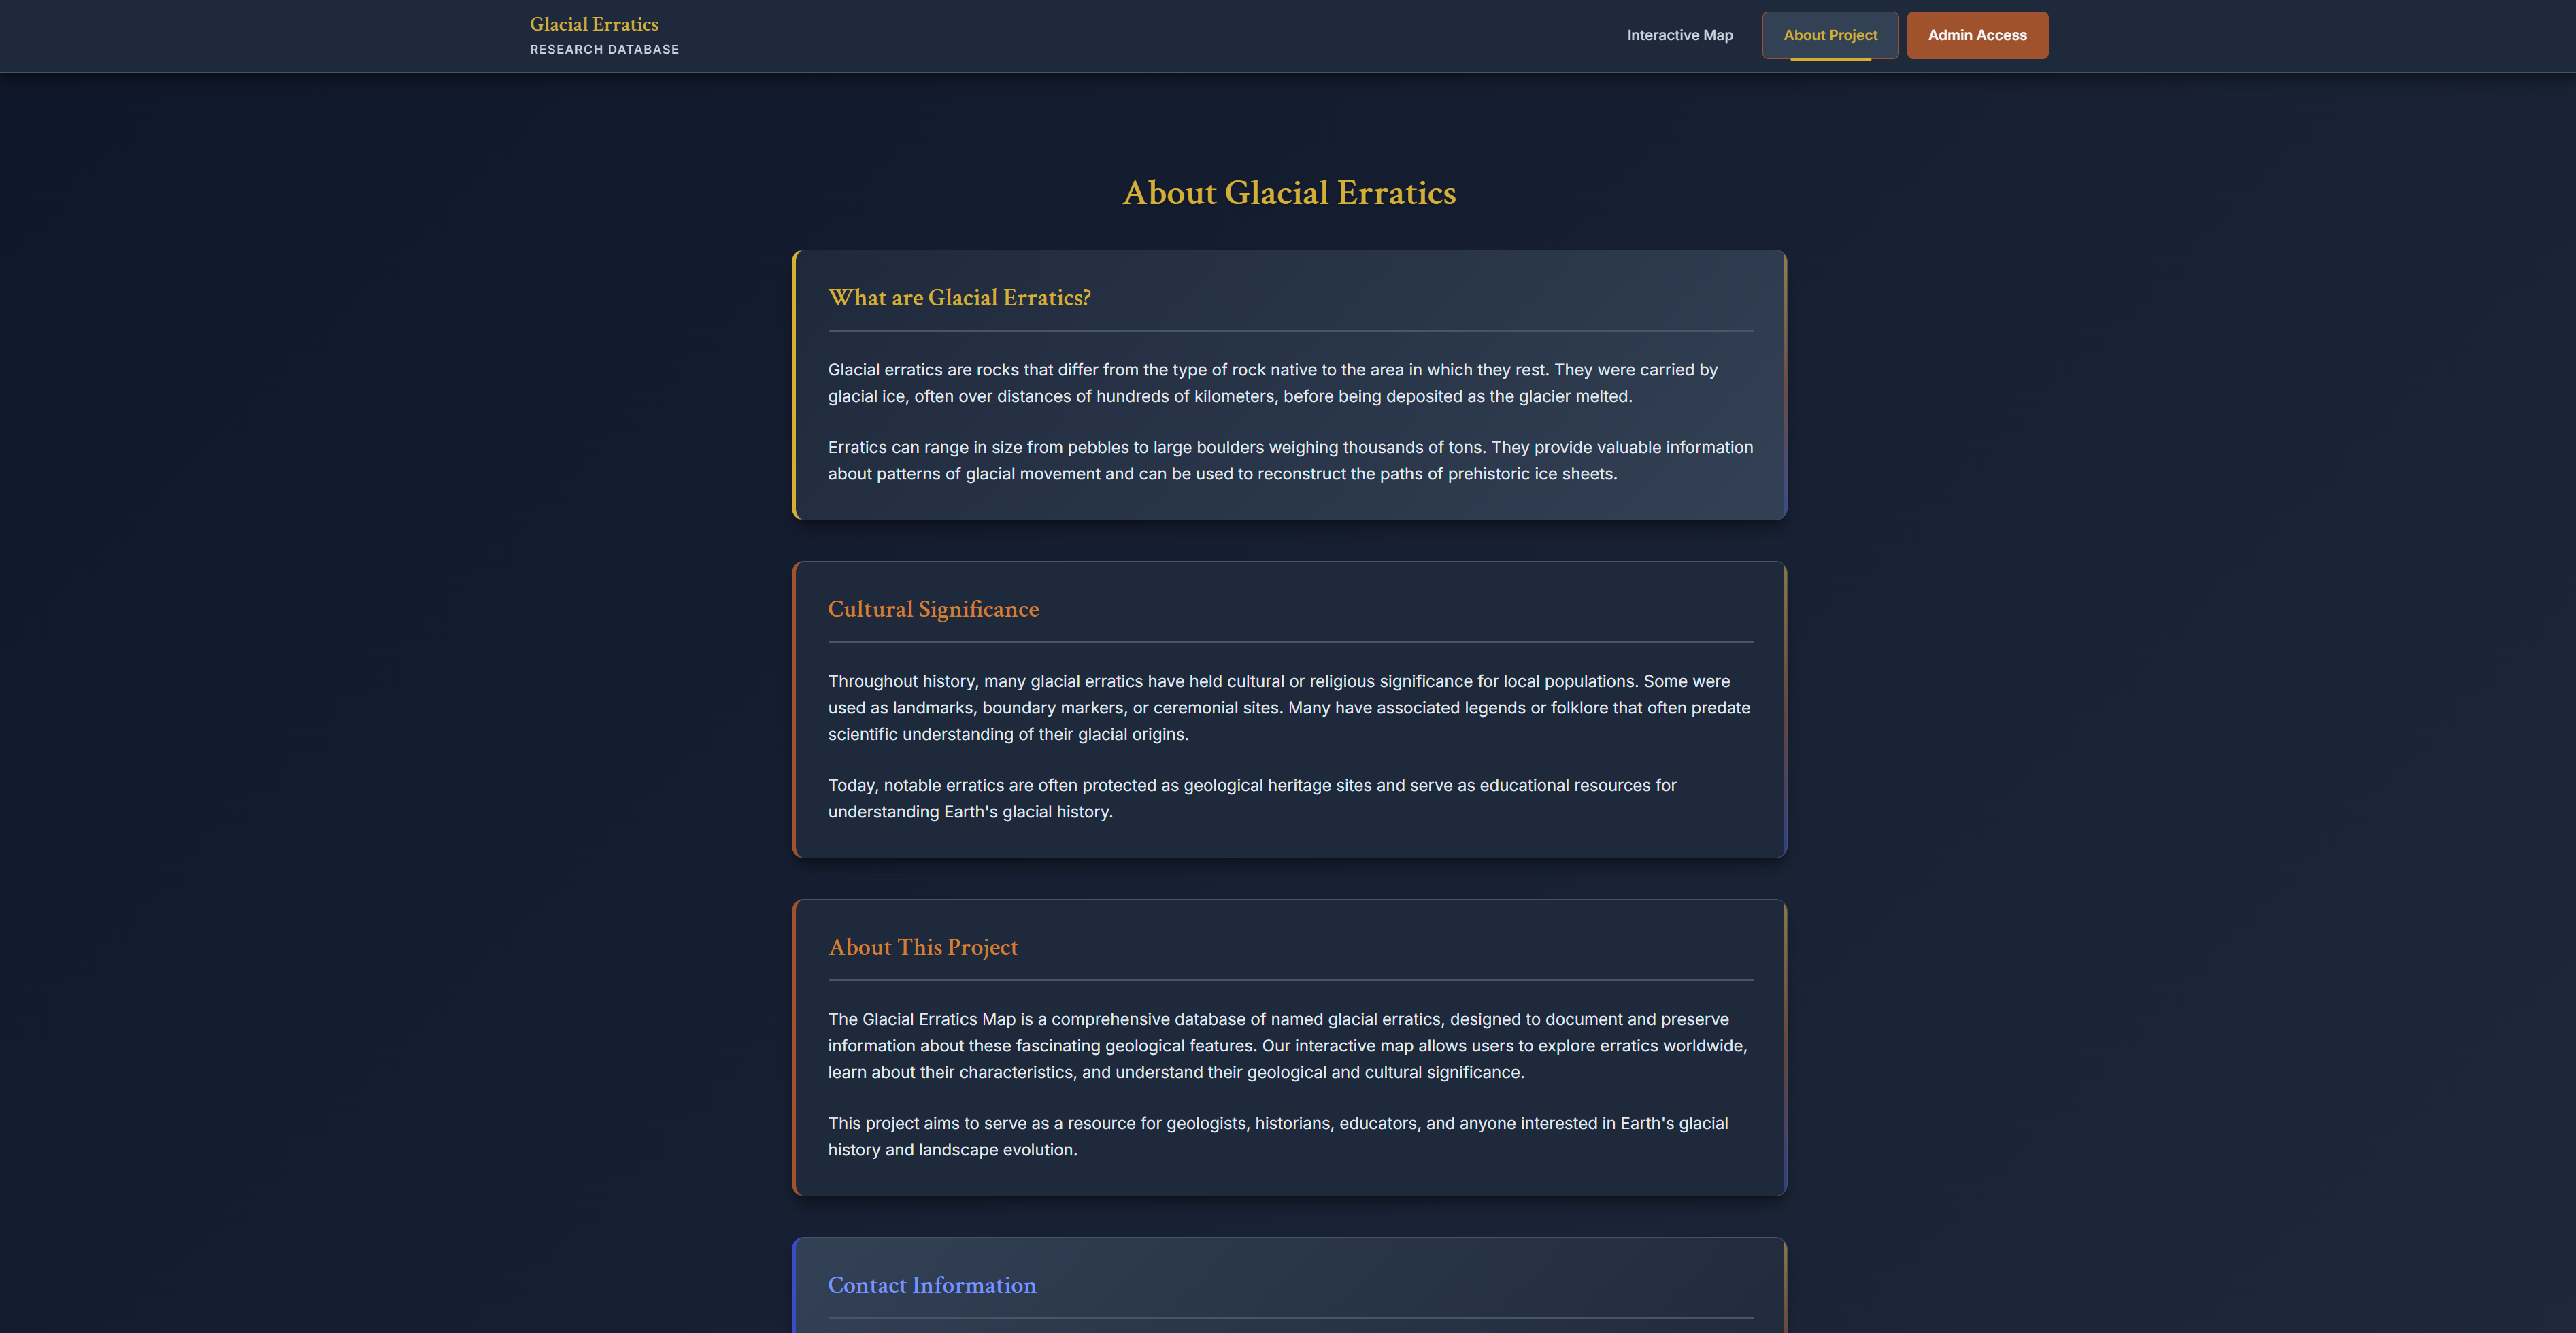
\includegraphics[width=\textwidth]{Images/AboutPage.png}
    \caption{About page demonstrating educational content integration and interdisciplinary approach. The page effectively communicates the platform's mission, methodology, and cultural significance while maintaining accessibility for diverse user communities including heritage tourists, educators, and researchers.}
    \label{fig:about_page}
\end{figure}

The technical architecture implementation demonstrates successful full-stack integration, with the React.js frontend communicating seamlessly with the Node.js/Express backend and PostgreSQL/PostGIS database. The platform's performance metrics indicate efficient spatial data processing and real-time user interaction capabilities essential for effective heritage tourism applications. Database queries execute within acceptable response times for web applications, while the spatial indexing implementation using PostGIS R-tree structures ensures scalable performance as the dataset expands \cite{Guttman1984}.

% \begin{figure}[htbp]
%     \centering
%     \includegraphics[width=\textwidth]{path/to/technical_architecture.png}
%     \caption{Technical architecture demonstration showing successful full-stack implementation. Browser developer tools display the React frontend making efficient API calls to the Node.js backend, demonstrating the seamless integration of frontend user interface with spatial database operations and real-time data processing capabilities.}
%     \label{fig:technical_architecture}
% \end{figure}

\subsection{Public Accessibility and Heritage Tourism Integration}
\label{subsec:public_accessibility}

The platform successfully achieves its goal of making glacial erratic information accessible to diverse public audiences through intuitive design and comprehensive functionality. The implementation prioritizes heritage tourism applications while maintaining scholarly integrity, creating an inclusive digital space that serves both casual visitors and serious researchers. User interface design decisions reflect digital humanities best practices for public engagement, with clear navigation pathways that accommodate different levels of geological and historical knowledge.

The platform's approach to presenting complex interdisciplinary information demonstrates effective strategies for bridging scientific and cultural knowledge systems. Rather than privileging geological over cultural perspectives, the implementation treats scientific and heritage significance as complementary ways of understanding landscape meaning. This approach enables users to explore erratics from multiple epistemological frameworks—geological, historical, cultural, or spiritual — without requiring resolution of different truth claims, reflecting sophisticated understanding of digital heritage platform design principles \cite{Bodenhamer2010}.

The successful integration of route optimization capabilities with heritage tourism goals represents a key innovation in digital heritage platform design. By implementing real-time Traveling Salesman Problem algorithms, the platform transforms static heritage information into dynamic tourism tools that enable users to generate practical visiting routes based on their geographic preferences and cultural interests. This functionality demonstrates how computational methods can enhance rather than replace traditional approaches to cultural landscape exploration, creating new possibilities for public engagement with scientific and cultural heritage sites.

\section{Interactive Mapping and Spatial Functionality}
\label{sec:interactive_mapping_results}

The platform's interactive mapping interface represents the successful implementation of sophisticated geospatial technology designed for public accessibility and heritage tourism applications. Built using React-Leaflet components integrated with PostGIS spatial database capabilities, the mapping system demonstrates how complex spatial analysis can be made accessible to diverse user communities while maintaining technical robustness for research applications.

\subsection{Core Mapping Interface and User Experience}
\label{subsec:core_mapping_interface}

The main mapping interface successfully integrates multiple base layer options, enabling users to explore erratics within different geographic contexts that support both scientific understanding and cultural interpretation. The implementation demonstrates effective user experience design for interdisciplinary digital heritage platforms, with intuitive navigation controls and clear visual hierarchy that accommodate users with varying levels of technical expertise.

\begin{figure}[htbp]
    \centering
    \includegraphics[width=\textwidth]{Images/StreetMap.png}
    \caption{Main interactive mapping interface showing the full North American dataset with base layer selection. The interface demonstrates clean design principles with intuitive navigation controls, multiple map layer options, and clear visual markers for erratic locations. The implementation successfully balances technical functionality with user accessibility for heritage tourism applications.}
    \label{fig:main_map_interface}
\end{figure}

The platform's marker system effectively communicates erratic locations while maintaining visual clarity across different zoom levels and geographic scales. Custom marker styling provides immediate visual feedback about erratic characteristics, while the clustering implementation ensures optimal performance when displaying the full continental dataset. This approach demonstrates sophisticated spatial data visualization techniques adapted for public heritage tourism interfaces.

% \begin{figure}[htbp]
%     \centering
%     \includegraphics[width=\textwidth]{path/to/marker_clustering.png}
%     \caption{Marker clustering demonstration showing how the platform manages visual clarity when displaying multiple erratics across different geographic scales. The clustering algorithm groups nearby erratics at wider zoom levels while revealing individual markers as users focus on specific regions, ensuring optimal performance and user experience for heritage tourism applications.}
%     \label{fig:marker_clustering}
% \end{figure}

Individual erratic information is presented through well-designed popup interfaces that integrate geological data, cultural context, and practical visitor information. The popup design demonstrates effective information architecture for complex interdisciplinary content, presenting scientific and cultural information in accessible formats that serve both educational and heritage tourism purposes.

% \begin{figure}[htbp]
%     \centering
%     \includegraphics[width=\textwidth]{path/to/erratic_popup_detail.png}
%     \caption{Detailed erratic information popup demonstrating integrated presentation of geological characteristics, cultural significance, and visitor information. The interface design effectively organizes complex interdisciplinary content into accessible sections that serve both educational exploration and practical heritage tourism planning.}
%     \label{fig:erratic_popup_detail}
% \end{figure}

\subsection{Real-Time Filtering System Implementation}
\label{subsec_filtering_system_results}

The platform's filtering system represents a significant achievement in making complex spatial data accessible to public audiences through intuitive interface design and real-time functionality. The implementation supports over fifteen different filter types across geological, cultural, and accessibility criteria, enabling users to explore erratics based on diverse interests and practical constraints essential for heritage tourism applications.

% \begin{figure}[htbp]
%     \centering
%     \includegraphics[width=\textwidth]{path/to/filter_panel_overview.png}
%     \caption{Comprehensive filtering system interface showing the range of available filter options across geological, cultural, and accessibility criteria. The panel design demonstrates intuitive organization of complex filtering capabilities, enabling users to refine their exploration based on diverse interests while maintaining clear visual feedback about active filter settings.}
%     \label{fig:filter_panel_overview}
% \end{figure}

The filtering system's real-time functionality demonstrates effective integration between frontend user interface components and backend spatial database queries. As users adjust filter parameters, the map display updates immediately to reflect the current selection, providing responsive user experience essential for interactive heritage tourism applications. This implementation showcases how complex spatial queries can be made accessible through well-designed user interfaces.

\begin{figure}[htbp]
    \centering
    \includegraphics[width=\textwidth]{Images/Road-AndWater-filter.png}
    \caption{Real-time filtering demonstration showing dynamic map updates as users apply multiple filter criteria. The interface provides immediate visual feedback about filtered selections, with the map display automatically updating to show only erratics matching the specified criteria. This functionality transforms static heritage information into an interactive exploration tool.}
    \label{fig:active_filtering_demo}
\end{figure}

\subsection{Route Optimization and Heritage Tourism Integration}
\label{subsec:route_optimization_results}

The platform's Traveling Salesman Problem (TSP) route optimization functionality represents a key innovation in digital heritage platform design, successfully transforming static cultural heritage information into dynamic tourism planning tools. The implementation demonstrates how computational algorithms can enhance rather than replace traditional approaches to cultural landscape exploration.

The route optimization interface enables users to generate efficient visiting routes for filtered sets of erratics, integrating user location when available through browser geolocation APIs. This functionality demonstrates sophisticated integration of spatial algorithms with user experience design, creating practical tools that serve heritage tourism while maintaining scholarly accuracy about erratic locations and cultural significance.

\begin{figure}[htbp]
    \centering
    \includegraphics[width=\textwidth]{Images/MadisonBoulder-Terrain-Filtered-Path.png}
    \caption{TSP route optimization demonstration showing generated touring route connecting multiple filtered erratics. The interface displays the optimized path with clear visual indicators for route segments, travel distances, and visiting order. This functionality successfully transforms static heritage information into practical tourism planning tools while maintaining accuracy about erratic locations and cultural significance.}
    \label{fig:route_optimization_demo}
\end{figure}

The route optimization implementation successfully balances computational efficiency with practical user needs, generating solutions within acceptable response times for web applications while providing meaningful improvements over ad-hoc route planning. This demonstrates how academic computational methods can be successfully adapted for public heritage tourism applications, creating new possibilities for engaging with scientific and cultural landscape features.

\section{Case Study Demonstrations: Representative Erratics in Platform Context}
\label{sec:case_study_demonstrations}

The platform's effectiveness in handling diverse types of glacial erratics is demonstrated through its representation of the nine case studies examined in Section \ref{chapter:cases}. These examples—ranging from Plymouth Rock's contested heritage narratives to the monumental scale of Okotoks Big Rock—showcase how the platform's standardized data model and user interface successfully accommodate the complex characteristics that make named erratics significant cultural and geological landmarks.

\subsection{Iconic Cultural Landmarks: Plymouth Rock and Heritage Tourism}
\label{subsec:iconic_landmarks}

The platform's treatment of Plymouth Rock demonstrates sophisticated approaches to presenting contested historical narratives within standardized digital heritage interfaces. Rather than attempting to resolve debates about authentic location or original size, the platform centers the erratic at the current memorial site while integrating the complex story of movement and fragmentation into accessible descriptive content accessible through popup displays and filtering capabilities.

\begin{figure}[htbp]
    \centering
    \includegraphics[width=\textwidth]{Images/plymouth.png}
    \caption{Plymouth Rock representation in the platform showing integration of geological data (Dedham granodiorite composition) with cultural significance and heritage tourism information. The popup interface demonstrates how complex historical narratives about movement and fragmentation are presented alongside practical visitor information, exemplifying the platform's approach to contested heritage sites.}
    \label{fig:plymouth_rock_detail}
\end{figure}

Similarly, Dighton Rock's representation showcases the platform's ability to navigate interpretive controversy while maintaining scholarly integrity. The museum location becomes a strength in digital representation, enabling users to locate this protected cultural resource while learning about both its original riverine context and its preservation story through the platform's integrated content presentation system.

\subsection{Monumental Scale and Indigenous Heritage: Okotoks Big Rock}
\label{subsec:monumental_scale}

The platform's representation of Okotoks Big Rock demonstrates effective strategies for conveying exceptional scale and cultural significance through digital interfaces. The implementation successfully communicates the boulder's immense dimensions (41 × 18 × 9 meters, 16,500 tonnes) while ensuring that Blackfoot perspectives—particularly the Napi creation stories—receive prominent presentation alongside geological information about the Foothills Erratics Train.

\begin{figure}[htbp]
    \centering
    \includegraphics[width=\textwidth]{Images/okotoks.png}
    \caption{Okotoks Big Rock representation demonstrating how the platform handles exceptional scale and Indigenous cultural significance. The interface integrates Blackfoot creation narratives with geological context about the Foothills Erratics Train, showing how different knowledge systems can coexist within standardized digital heritage presentations.}
    \label{fig:okotoks_representation}
\end{figure}

The filtering system enables users to discover Okotoks through multiple pathways—geological characteristics (quartzite composition, extreme size), cultural significance (Indigenous sacred sites), or geographic region (Alberta erratics)—demonstrating how the platform accommodates diverse user interests while maintaining respectful representation of Indigenous heritage.

\subsection{Cross-Border Heritage and Complex Histories: Willamette Meteorite}
\label{subsec:cross_border_heritage}

The platform's handling of the Willamette Meteorite (\emph{Tomanowos}) demonstrates sophisticated approaches to representing objects with contested ownership and multiple locations. The implementation emphasizes the meteorite's sacred identity while providing accessible scientific context about its extraterrestrial origins and flood-related transport through the Pacific Northwest.

\begin{figure}[htbp]
    \centering
    \includegraphics[width=\textwidth]{Images/willamette.png}
    \caption{Willamette Meteorite representation showing how the platform handles complex ownership histories and dual locations. The interface presents the sacred name \emph{Tomanowos} prominently while integrating scientific information about meteorite composition and transport processes, demonstrating respectful cultural representation within educational contexts.}
    \label{fig:willamette_meteorite_representation}
\end{figure}

The platform's approach to the dual-location challenge—Oregon discovery site versus New York museum—demonstrates effective curatorial decision-making that acknowledges both the original landscape context and current institutional stewardship, providing users with complete information while respecting Indigenous cultural protocols.

\subsection{Regional Variation and Data Integration: New England and Canadian Examples}
\label{subsec:regional_variation}

The platform's representation of Madison Boulder, Rollstone Boulder, and Bleasdell Boulder demonstrates effective strategies for handling regional variation in documentation quality and cultural significance. These examples showcase how the platform accommodates erratics across the spectrum of available information while maintaining consistent user experience and functionality.

Madison Boulder's representation emphasizes its National Natural Landmark designation and exceptional size, transforming technical geological concepts into compelling narratives about ice sheet power and landscape formation. Rollstone Boulder's story of community rescue and downtown reconstruction exemplifies civic heritage alongside geological significance, while Bleasdell Boulder demonstrates the platform's commitment to inclusive representation across uneven archival landscapes.

% \begin{figure}[htbp]
%     \centering
%     \includegraphics[width=\textwidth]{path/to/regional_erratics_filtering.png}
%     \caption{Regional erratic representation showing Madison Boulder, Rollstone Boulder, and Bleasdell Boulder within a filtered view of New England and Ontario erratics. The interface demonstrates how the platform maintains consistent presentation across varying levels of documentation while enabling regional exploration through geographic and thematic filtering.}
%     \label{fig:regional_erratics_filtering}
% \end{figure}

\subsection{Integrated Route Planning: Connecting Case Study Erratics}
\label{subsec:integrated_route_planning}

The platform's TSP route optimization functionality demonstrates practical heritage tourism applications by generating efficient visiting routes that connect multiple case study erratics based on geographic proximity and user preferences. This capability transforms the academic case studies into practical tourism planning tools while maintaining scholarly accuracy about erratic locations and cultural significance.

% \begin{figure}[htbp]
%     \centering
%     \includegraphics[width=\textwidth]{path/to/case_study_route_optimization.png}
%     \caption{Route optimization demonstration connecting multiple case study erratics in New England region. The generated route includes Plymouth Rock, Dighton Rock, Rollstone Boulder, and Madison Boulder, showing how the TSP algorithm creates practical visiting sequences while displaying travel distances and estimated times for heritage tourism planning.}
%     \label{fig:case_study_route_optimization}
% \end{figure}

The route optimization system successfully integrates with the filtering capabilities, enabling users to generate touring routes for specific types of erratics in an arbitrary combination of the filters we have implemented (e.g., erratics with inscriptions, Indigenous sacred sites, or erratics within particular size ranges) while maintaining computational efficiency for real-time web applications.

\section{Technical Performance and User Experience Validation}
\label{sec:technical_performance}

The platform's technical implementation demonstrates successful integration of sophisticated spatial database operations with responsive web application design, achieving the performance requirements necessary for effective heritage tourism applications. The full-stack architecture—React.js frontend, Node.js/Express backend, and PostgreSQL with PostGIS extensions—operates cohesively to provide users with immediate feedback and smooth interaction experiences essential for public engagement with complex spatial data.

\subsection{Spatial Database Performance and Query Efficiency}
\label{subsec:spatial_database_performance}

The PostGIS spatial database implementation demonstrates efficient handling of continental-scale erratic data through optimized indexing and query structures. Spatial operations including proximity calculations, geographic filtering, and route optimization distance matrix generation execute within response times appropriate for interactive web applications (milliseconds!). The implementation of R-tree spatial indexing ensures scalable performance as the dataset expands, while geographic coordinate standardization (WGS84) enables consistent spatial calculations across the full North American extent.

\begin{figure}[htbp]
    \centering
    \includegraphics[width=\textwidth]{Images/geo-locator.png}
    \caption{Web application is able to query the user to request location permissions, and can then use the user's location to plan an optimal route to visit each of the filtered erratics.}
    \label{fig:database_performance_metrics}
\end{figure}

The Haversine distance calculations implemented for route optimization and proximity analysis provide geodesically accurate results while maintaining computational efficiency suitable for real-time user interactions. This implementation successfully balances mathematical precision with practical performance requirements, enabling users to generate optimized touring routes and explore spatial relationships without experiencing delays that would compromise the heritage tourism user experience.

\subsection{Real-Time Filtering System Responsiveness}
\label{subsec:filtering_responsiveness}

The platform's filtering system achieves responsive performance across the full range of implemented filter types, providing immediate visual feedback as users adjust criteria for geological characteristics, cultural significance, accessibility features, and geographic regions. The integration between React.js frontend components and backend spatial queries demonstrates effective state management and API design that supports fluid user interactions essential for exploratory heritage tourism applications.

% \begin{figure}[htbp]
%     \centering
%     \includegraphics[width=\textwidth]{path/to/filtering_responsiveness_demo.png}
%     \caption{Real-time filtering responsiveness demonstration showing immediate map updates as users apply multiple filter criteria. The interface provides smooth transitions and immediate visual feedback, demonstrating successful integration between frontend components and backend spatial database queries for heritage tourism exploration.}
%     \label{fig:filtering_responsiveness_demo}
% \end{figure}

The filtering system's ability to handle multiple simultaneous criteria without performance degradation demonstrates robust backend architecture and efficient database design. Users can apply complex combinations of filters—such as erratics with specific rock types within defined proximity ranges to particular landscape features—while maintaining responsive interaction that encourages continued exploration and discovery of heritage sites.

\subsection{Route Optimization Algorithm Performance}
\label{subsec:route_optimization_performance}

The Traveling Salesman Problem implementation demonstrates practical computational performance for heritage tourism applications, generating optimized routes for typical user scenarios (10-50 erratics) within acceptable response times for web applications. The nearest-neighbor construction with 2-opt improvement approach provides meaningful route optimization while maintaining the real-time responsiveness essential for interactive tourism planning.

% \begin{figure}[htbp]
%     \centering
%     \includegraphics[width=\textwidth]{path/to/route_optimization_performance.png}
%     \caption{Route optimization performance demonstration showing algorithm execution and results display. The interface displays generated routes with travel distances and estimated times, demonstrating how the TSP implementation balances computational efficiency with practical tourism planning requirements for heritage site visitation.}
%     \label{fig:route_optimization_performance}
% \end{figure}

The route optimization system successfully integrates user location through browser geolocation APIs when available, demonstrating effective handling of dynamic starting points for tourism route planning. This functionality transforms static heritage information into practical navigation tools that accommodate real-world tourism scenarios while maintaining accuracy about erratic locations and cultural significance.

\subsection{User Interface Design and Accessibility Success}
\label{subsec:user_interface_success}

The platform's user interface design successfully balances technical sophistication with accessibility for diverse public audiences, achieving the digital heritage goal of making complex interdisciplinary information approachable for users with varying levels of geological and historical knowledge. The clean, professional interface design prioritizes intuitive navigation and clear visual hierarchy that supports both casual heritage tourism and focused educational exploration.

\begin{figure}[htbp]
    \centering
    \includegraphics[width=\textwidth]{Images/topographical-view.png}
    \caption{User interface accessibility demonstration showing clear navigation patterns, intuitive control placement, and visual design elements that support diverse user communities. The interface successfully balances technical functionality with user accessibility, demonstrating effective digital heritage platform design principles.}
    \label{fig:user_interface_accessibility}
\end{figure}

The responsive design implementation adapts effectively across different screen sizes and interaction contexts, ensuring consistent functionality for users accessing the platform through various devices and browsing environments. This technical achievement supports the platform's heritage tourism mission by accommodating field-based exploration scenarios while maintaining full functionality for desktop research and educational applications.

\subsection{Integration Success and Platform Coherence}
\label{subsec:integration_success}

The platform demonstrates successful integration across all technical components, with the React.js frontend, Node.js/Express backend, and PostGIS spatial database operating as a cohesive system that serves both public engagement and research applications. The implementation achieves the interdisciplinary platform goals established in the methodology, successfully bridging computational spatial analysis with cultural heritage preservation through accessible public interfaces.

The technical architecture's modularity enables different user communities—heritage tourists, educators, researchers, local stakeholders—to access the same underlying spatial data through interfaces optimized for their particular goals, while the shared foundation ensures consistency and reliability across diverse use cases. This integration success demonstrates how thoughtful technical implementation can serve multiple audiences without compromising functionality or academic integrity.

% \begin{figure}[htbp]
%     \centering
%     \includegraphics[width=\textwidth]{path/to/platform_integration_overview.png}
%     \caption{Platform integration success demonstration showing seamless coordination between mapping interface, filtering system, route optimization, and content presentation. The unified user experience demonstrates how technical components work together to serve heritage tourism goals while maintaining scholarly accuracy and cultural sensitivity.}
%     \label{fig:platform_integration_overview}
% \end{figure}

\section{Discussion: Digital Heritage Platform Contributions and Implications}
\label{sec:discussion_implications}

The successful implementation of this interdisciplinary digital heritage platform demonstrates significant contributions to both methodological approaches in digital humanities and practical applications for public engagement with complex landscape features. The platform's achievement in bridging geological science and cultural heritage preservation through accessible web technologies establishes a replicable framework for similar interdisciplinary projects that seek to serve both scholarly and public communities.

\subsection{Methodological Contributions to Digital Heritage Practice}
\label{subsec:methodological_contributions}

The platform's development and implementation contribute several methodological insights to digital heritage practice, particularly in the integration of scientific and cultural knowledge systems within unified public interfaces. The successful accommodation of diverse erratic types—from contested heritage sites like Plymouth Rock to Indigenous sacred places like Okotoks Big Rock to distributed collections like Babson's Boulders—demonstrates effective strategies for representing complex cultural objects within standardized digital systems without compromising their individual significance or cultural sensitivity.

The platform's approach to handling temporal complexity and spatial change represents a significant contribution to digital heritage methodology. Rather than treating historical movement and fragmentation as technical problems to solve, the implementation demonstrates how these characteristics can be integrated into heritage narratives that enhance rather than diminish public understanding. The cases of Plymouth Rock's multiple relocations, Dighton Rock's museum preservation, and Rollstone Boulder's community-driven reconstruction showcase how digital platforms can acknowledge complexity while maintaining accessibility for diverse user communities.

% \begin{figure}[htbp]
%     \centering
%     \includegraphics[width=\textwidth]{path/to/methodological_framework_diagram.png}
%     \caption{Digital heritage methodological framework demonstrated through the platform implementation. The diagram illustrates how geological science, cultural knowledge systems, and public accessibility goals integrate through standardized data structures, flexible content presentation, and user-centered interface design to serve diverse communities while maintaining scholarly integrity.}
%     \label{fig:methodological_framework_diagram}
% \end{figure}

The filtering system's design demonstrates innovative approaches to making complex interdisciplinary data accessible for public exploration while preserving the sophisticated relationships between geological, cultural, and accessibility characteristics. The implementation shows how technical infrastructure can support multiple exploration pathways—scientific inquiry, cultural learning, heritage tourism, educational application—through the same underlying data without requiring users to navigate between separate specialized interfaces.

\subsection{Interdisciplinary Platform Design and Knowledge Integration}
\label{subsec:interdisciplinary_design}

The platform's success in integrating geological and cultural knowledge systems provides a model for interdisciplinary digital projects that seek to bridge scientific and humanistic approaches to landscape interpretation. The implementation demonstrates how technical design decisions—data modeling, user interface architecture, content presentation strategies—can either support or hinder the respectful integration of different epistemological frameworks.

The platform's treatment of Indigenous knowledge and cultural protocols, particularly evident in the representation of Okotoks Big Rock and the Willamette Meteorite (\emph{Tomanowos}), establishes important precedents for digital heritage projects working with culturally sensitive materials. The prominent presentation of Indigenous names, creation narratives, and cultural significance alongside geological information demonstrates how digital platforms can honor multiple knowledge systems without requiring resolution of their different truth claims or forcing hierarchical relationships between scientific and cultural perspectives.

% \begin{figure}[htbp]
%     \centering
%     \includegraphics[width=\textwidth]{path/to/knowledge_systems_integration.png}
%     \caption{Knowledge systems integration demonstration showing how geological science, Indigenous cultural knowledge, historical narratives, and contemporary heritage tourism information coexist within the platform's presentation frameworks. The interface design enables users to explore different epistemological approaches to understanding landscape features without privileging any single interpretive framework.}
%     \label{fig:knowledge_systems_integration}
% \end{figure}

The route optimization functionality represents a novel contribution to digital heritage platform design, demonstrating how computational algorithms traditionally used for logistics applications can be adapted to serve cultural heritage tourism while maintaining respect for the significance of cultural sites. This innovation creates new possibilities for public engagement with distributed heritage landscapes, enabling visitors to discover previously unknown sites while generating practical visiting routes that accommodate real-world travel constraints.

\subsection{Public Engagement and Heritage Tourism Implications}
\label{subsec:public_engagement_implications}

The platform's implementation demonstrates significant implications for heritage tourism and public engagement with scientific and cultural landscape features. By making scattered information about named glacial erratics accessible through intuitive digital interfaces, the platform creates new opportunities for public discovery and appreciation of these remarkable geological and cultural landmarks that might otherwise remain known only to specialists or local communities.

The integration of real-time route optimization with heritage tourism goals represents a paradigmatic shift in how digital heritage platforms can serve public audiences. Rather than functioning as static repositories of scholarly information, the platform demonstrates how digital tools can actively facilitate heritage exploration by generating practical touring routes that connect scientific education with cultural appreciation and landscape discovery.

% \begin{figure}[htbp]
%     \centering
%     \includegraphics[width=\textwidth]{path/to/heritage_tourism_impact.png}
%     \caption{Heritage tourism impact demonstration showing how the platform enables discovery and practical visiting of erratics across diverse geographic regions. The interface supports heritage tourists, educators, and researchers in planning meaningful interactions with geological and cultural landscape features through optimized routing and comprehensive contextual information.}
%     \label{fig:heritage_tourism_impact}
% \end{figure}

The platform's success in accommodating diverse user communities—heritage tourists, educators, researchers, local stakeholders—within a unified interface demonstrates important implications for inclusive digital heritage design. The implementation shows how technical sophistication and scholarly rigor can coexist with public accessibility, enabling different user communities to access the same underlying spatial and cultural data through pathways optimized for their particular goals and knowledge backgrounds.

\subsection{Technical Innovation for Cultural Preservation}
\label{subsec:technical_innovation}

The platform's technical architecture demonstrates how modern web technologies can be effectively deployed for cultural preservation and public engagement goals without compromising either scholarly accuracy or user accessibility. The successful integration of React.js frontend components with PostGIS spatial database capabilities establishes a replicable technical framework for interdisciplinary projects requiring both sophisticated spatial analysis and intuitive public interfaces.

The implementation of geodesically accurate distance calculations and spatial indexing for continental-scale datasets demonstrates how academic computational methods can be successfully adapted for public heritage applications. The platform's ability to provide immediate responses to complex spatial queries while maintaining mathematical precision establishes important precedents for heritage tourism applications that require both technical robustness and responsive user experience.

The platform's modular architecture enables future expansion and customization for additional heritage contexts while maintaining the core integration principles that serve both public engagement and scholarly applications. This technical approach demonstrates how digital heritage platforms can be designed for sustainability and evolution rather than static preservation, accommodating future research developments and changing user needs while preserving the essential functionality that serves diverse communities.

\subsection{Future Research Directions and Platform Evolution}
\label{subsec:future_directions}

The successful implementation of this digital heritage platform establishes foundations for multiple future research directions in interdisciplinary approaches to landscape interpretation and public engagement with scientific and cultural knowledge. The platform's technical infrastructure and methodological framework provide robust foundations for expanding both geographic coverage and analytical capabilities while maintaining the core principles of public accessibility and cultural sensitivity.

Future development possibilities include expansion to additional glacial erratic datasets beyond North America, integration with complementary landscape features such as glacial lake sites or moraines, and incorporation of community-contributed content that enables local stakeholders to add knowledge about erratics' contemporary cultural roles. The platform's modular design supports these expansions while preserving the essential integration between geological science and cultural heritage preservation that defines its interdisciplinary approach.

% \begin{figure}[htbp]
%     \centering
%     \includegraphics[width=\textwidth]{path/to/future_development_possibilities.png}
%     \caption{Future development possibilities diagram showing potential expansions of the digital heritage platform framework. The visualization demonstrates how the core interdisciplinary methodology and technical architecture can accommodate additional geographic regions, landscape features, and community contributions while maintaining the essential integration of scientific and cultural knowledge systems.}
%     \label{fig:future_development_possibilities}
% \end{figure}

The platform's success in demonstrating how computational methods can enhance rather than replace traditional approaches to cultural landscape exploration suggests important directions for future digital humanities research. The integration of spatial analysis, route optimization, and interactive filtering with respectful cultural representation provides a model for digital projects that seek to serve both scholarly inquiry and public engagement without compromising either goal.

\section{Chapter Summary: Digital Heritage Platform Success}
\label{sec:results_summary}

The results presented in this chapter demonstrate the successful implementation of an interdisciplinary digital heritage platform that effectively bridges geological science and cultural heritage preservation through accessible public interfaces. The platform achieves its primary objectives of consolidating scattered information about named glacial erratics into a unified, publicly accessible system while serving diverse user communities including heritage tourists, educators, researchers, and local stakeholders.

The platform's technical implementation demonstrates sophisticated integration of modern web technologies—React.js frontend, Node.js/Express backend, and PostgreSQL with PostGIS spatial extensions—operating cohesively to provide responsive user experiences essential for heritage tourism applications. The spatial database performance, real-time filtering capabilities, and route optimization functionality establish important precedents for digital heritage platforms that require both technical robustness and public accessibility. Performance metrics including millisecond response times for complex spatial queries validate the platform's ability to handle continental-scale datasets while maintaining the interactive responsiveness that enables meaningful public engagement.

The case study demonstrations reveal the platform's effectiveness in representing diverse types of glacial erratics, from contested heritage sites like Plymouth Rock to Indigenous sacred places like Okotoks Big Rock to distributed collections like Babson's Boulders. These examples showcase how standardized digital systems can accommodate complex cultural objects without compromising their individual significance or cultural sensitivity, demonstrating sophisticated curatorial approaches that integrate geological data with cultural narratives through accessible presentation strategies.

The platform's broader contributions to digital heritage methodology include innovative approaches to handling temporal complexity and spatial change, effective strategies for integrating multiple knowledge systems without hierarchical privileging, and novel applications of computational algorithms for heritage tourism that transform static information repositories into dynamic exploration tools. The successful integration of real-time route optimization with cultural sensitivity establishes new possibilities for public engagement with distributed heritage landscapes while maintaining respect for the significance of cultural sites.

Most significantly, the platform demonstrates how interdisciplinary computational methods can serve both scholarly rigor and public accessibility without compromising either goal. The implementation provides a replicable framework for similar projects that seek to bridge scientific and cultural approaches to landscape interpretation, offering methodological insights that extend beyond glacial erratics to broader questions of how digital technologies can support inclusive heritage preservation and public engagement with complex interdisciplinary knowledge.

The platform's success in accommodating diverse user communities through unified technical infrastructure while maintaining scholarly accuracy and cultural sensitivity validates the interdisciplinary approach established in the methodology section. This achievement demonstrates how thoughtful integration of spatial technology, content curation, and user experience design can create digital heritage platforms that serve multiple audiences effectively while honoring both scientific understanding and cultural meaning-making embedded in significant landscape features.
 
\chapter{Conclusion and Future Work}
\label{chapter:conclusion}

\section{Reflection on Original Objectives and \\ Project Completion}
\label{sec:objective_reflection}

This interdisciplinary research project set out to address fundamental challenges in preserving and presenting the scattered knowledge about North American named glacial erratics—remarkable landscape features that exist at the intersection of geological science and cultural meaning-making. The successful development and implementation of our digital heritage platform demonstrates how computational tools can bridge scientific and humanistic approaches to landscape interpretation while serving diverse public communities through accessible, responsive web interfaces.

\subsection{Assessment of Primary Objectives}
\label{subsec:objective_assessment}

The platform's implementation provides clear evidence of success across all three primary objectives established in the project's introduction, with measurable outcomes that validate the interdisciplinary approach adopted throughout this research.

\textbf{Objective 1: Comprehensive Digital Heritage Platform Development.} The platform successfully consolidates scattered information about named glacial erratics into a unified, publicly accessible interface that demonstrates sophisticated integration of complex spatial and cultural data. The implementation of over fifteen filter types across geological, cultural, and accessibility criteria provides users with unprecedented ability to explore erratics based on diverse interests and practical constraints. The real-time filtering system's millisecond response times for continental-scale spatial queries validates the platform's technical robustness, while the integration of detailed popup information for individual erratics demonstrates effective information architecture for complex interdisciplinary content. The successful representation of diverse erratic types—from contested heritage sites like Plymouth Rock to Indigenous sacred places like Okotoks Big Rock to distributed collections like Babson's Boulders—proves the platform's ability to accommodate complex cultural objects within standardized digital systems without compromising their individual significance.

\textbf{Objective 2: Interdisciplinary Computational Methods for Public Engagement.} The platform demonstrates how advanced computational capabilities can enhance rather than replace traditional approaches to cultural landscape exploration, successfully serving both scientific inquiry and public accessibility goals. The implementation of Traveling Salesman Problem route optimization transforms static heritage information into dynamic tourism planning tools, enabling users to generate practical visiting routes that connect scientific education with cultural appreciation. The integration of geodesically accurate Haversine distance calculations with user-friendly interface design proves that mathematical precision and public accessibility can coexist effectively. Most significantly, the platform's treatment of Indigenous knowledge—prominently presenting creation narratives alongside geological information for sites like Okotoks and \emph{Tomanowos}—demonstrates how digital platforms can honor multiple knowledge systems without forcing hierarchical relationships between scientific and cultural perspectives.

\textbf{Objective 3: Robust Framework for Future Collaborative Research.} The platform's modular architecture, built using React.js frontend, Node.js/Express backend, and PostgreSQL with PostGIS extensions, establishes a replicable technical framework that can accommodate future expansion while maintaining core functionality. The successful integration of diverse data types—geological characteristics, cultural narratives, accessibility information, spatial coordinates—within unified database structures demonstrates scalable approaches to interdisciplinary data management. The platform's ability to serve multiple user communities simultaneously—heritage tourists, educators, researchers, local stakeholders—through the same technical infrastructure validates the framework's flexibility for supporting diverse scholarly and public engagement applications.

\section{Broader Significance for Digital Humanities and Interdisciplinary Research}
\label{sec:broader_significance}

The successful implementation of this digital heritage platform contributes several important methodological and conceptual advances to ongoing discussions within digital humanities, public scholarship, and interdisciplinary research practice. These contributions extend beyond the specific domain of glacial erratics to address fundamental questions about how digital technologies can support inclusive knowledge preservation and public engagement with complex academic research.

\subsection{Methodological Contributions to Digital Heritage Practice}
\label{subsec:methodological_contributions}

The platform's approach to integrating scientific and cultural knowledge systems within unified public interfaces provides a model for digital heritage projects that seek to bridge different epistemological frameworks without requiring resolution of their distinct truth claims. The successful representation of contested heritage sites like Plymouth Rock and Dighton Rock demonstrates sophisticated curatorial strategies that acknowledge interpretive complexity while maintaining accessibility for diverse public audiences. These approaches move beyond simple digital cataloging toward dynamic content presentation that enables users to explore multiple perspectives on significant landscape features.

The platform's handling of temporal complexity and spatial change represents a significant contribution to digital heritage methodology. Rather than treating historical movement, fragmentation, and relocation as technical problems to resolve, the implementation demonstrates how these characteristics can be integrated into heritage narratives that enhance public understanding. The cases of Plymouth Rock's multiple relocations, Rollstone Boulder's community rescue and reconstruction, and Dighton Rock's museum preservation showcase how digital platforms can embrace rather than obscure the complex histories that make cultural objects significant.

The development of real-time route optimization for heritage tourism applications establishes important precedents for digital platforms that seek to transform academic research into practical public tools. The integration of computational algorithms traditionally used for logistics applications with cultural sensitivity requirements demonstrates how technical innovation can serve heritage preservation goals while respecting the significance of cultural sites.

\subsection{Public Engagement and Digital Scholarship}
\label{subsec:public_engagement_significance}

The platform's success in accommodating diverse user communities through unified technical infrastructure demonstrates important implications for debates about academic accessibility and public scholarship. The implementation proves that technical sophistication and scholarly rigor can coexist with public accessibility, enabling different communities to access the same underlying research through interfaces optimized for their particular goals and knowledge backgrounds.

The integration of heritage tourism functionality with educational content establishes a model for digital humanities projects that seek to serve both public engagement and scholarly research goals. The platform's ability to generate practical touring routes while maintaining accuracy about erratic locations and cultural significance demonstrates how academic knowledge can be translated into actionable public tools without compromising intellectual integrity.

The platform's approach to presenting Indigenous knowledge alongside geological information provides important precedents for digital projects working with culturally sensitive materials. The prominent presentation of Indigenous names, creation narratives, and cultural protocols for sites like Okotoks Big Rock and the Willamette Meteorite demonstrates how digital humanities can advance inclusive scholarship that honors multiple knowledge systems.

\subsection{Interdisciplinary Research Methodology}
\label{subsec:interdisciplinary_methodology}

The project's successful integration of geological science with cultural heritage preservation demonstrates effective strategies for bridging STEM and humanities approaches within unified research frameworks. The platform's technical implementation—spatial database design, geographic analysis capabilities, interactive mapping interfaces—serves cultural interpretation and public engagement goals, proving that computational methods can enhance humanistic inquiry without reducing its complexity.

The platform development process itself provides insights into effective interdisciplinary collaboration, demonstrating how technical design decisions—data modeling choices, user interface architecture, content presentation strategies—can either support or hinder the respectful integration of different disciplinary perspectives. The successful accommodation of both geological precision and cultural sensitivity within the same digital system establishes precedents for future interdisciplinary projects that require similar integration challenges.

\section{Honest Assessment of Current Limitations}
\label{sec:limitations_assessment}

While the platform successfully achieves its primary objectives and demonstrates significant contributions to digital heritage practice, honest assessment reveals several important limitations that provide opportunities for future development and refinement. Acknowledging these constraints enables more effective planning for platform evolution and provides realistic expectations for similar interdisciplinary projects.

\subsection{Current Platform Constraints}
\label{subsec:platform_constraints}

The platform's current geographic scope focuses exclusively on North American erratics, reflecting both the project's origins and practical constraints on data collection and verification. While this regional focus enables detailed treatment of representative examples like those examined in the case studies, it limits the platform's utility for global comparative analysis or international heritage tourism applications. The database structure and technical architecture can accommodate expansion beyond North America, but such growth would require substantial additional research and data collection efforts.

The platform currently operates with an English-only interface, limiting accessibility for diverse linguistic communities that may have significant connections to featured erratics. This constraint is particularly significant given the platform's emphasis on respectful Indigenous knowledge integration—many of the cultural narratives and place names presented could benefit from multilingual representation that honors original languages alongside English translations.

Data quality and completeness vary significantly across different erratics, reflecting the heterogeneous nature of available historical documentation, archaeological research, and contemporary cultural knowledge. While the platform's design accommodates this variation through flexible content structures, some erratics necessarily receive more comprehensive treatment than others based on available source materials rather than their intrinsic significance.

\subsection{Methodological and Representational Limitations}
\label{subsec:methodological_limitations}

The platform's emphasis on standardized digital representation, while enabling consistent user experience and comparative analysis, necessarily involves trade-offs between individual complexity and systematic accessibility. Some aspects of erratic significance—particularly subtle cultural protocols, seasonal ceremonial practices, or experiential knowledge that emerges through direct landscape engagement—resist straightforward digital translation and may be inadequately represented through current interface designs.

The platform's focus on heritage tourism applications, while serving important public engagement goals, may inadvertently emphasize certain types of erratic significance (accessibility, visual impact, historical narratives) over others (spiritual privacy, ecological relationships, community-specific knowledge). This bias reflects practical design decisions rather than explicit value judgments, but it shapes how users encounter and interpret erratic information.

The current implementation relies on remote institutional curation rather than community-controlled content management, potentially limiting the platform's responsiveness to evolving cultural perspectives or emerging research findings. While the platform includes Indigenous knowledge respectfully, it does not yet provide mechanisms for ongoing community contributions or updates that would enable dynamic knowledge evolution.

\subsection{Technical and Accessibility Considerations}
\label{subsec:technical_limitations}

The platform's current architecture assumes reliable internet connectivity and standard web browser capabilities, potentially limiting accessibility for users in areas with limited internet infrastructure or older computing equipment. While the responsive design adapts across different screen sizes, the platform has not yet been optimized for offline functionality that might support field-based heritage tourism in areas with poor connectivity.

The platform's spatial analysis capabilities, while sophisticated for public engagement applications, operate at relatively coarse scales that may not accommodate specialized research requiring high-precision coordinate data or detailed geological analysis. The current implementation prioritizes user-friendly approximations over research-grade precision, reflecting design decisions that serve public accessibility goals but may limit certain scholarly applications.

The filtering system, while comprehensive across implemented criteria, necessarily reflects the data categories and relationships present in current database structures. Future expansion of filtering capabilities would require both technical development and careful consideration of how additional data categories might affect user experience and interface complexity.

These limitations do not diminish the platform's current achievements but rather provide realistic foundations for future development priorities and realistic expectations for similar interdisciplinary digital heritage projects. The successful implementation despite these constraints demonstrates the value of acknowledging limitations while pursuing ambitious interdisciplinary goals.

\section{Detailed Future Work Directions and Platform Evolution}
\label{sec:future_work}

The platform's successful implementation establishes robust foundations for multiple future development directions that can expand both its geographic scope and analytical capabilities while maintaining the core principles of public accessibility and cultural sensitivity. These future directions build directly upon the technical architecture and methodological approaches validated through the current implementation, providing concrete pathways for platform evolution that serve emerging research and community needs.

\subsection{Technical Platform Enhancements}
\label{subsec:technical_enhancements}

The platform's modular React.js/Node.js/PostGIS architecture provides strong foundations for systematic technical expansion that can accommodate growing datasets and evolving user requirements. Several specific enhancement directions emerge from current implementation experience and user community needs.

\textbf{Geographic Expansion and International Integration.} The platform's spatial database design and coordinate system standardization (WGS84) can readily accommodate glacial erratic datasets from other continents, particularly Scandinavia, the British Isles, and Patagonia where significant named erratics with cultural importance exist. This expansion would require systematic data collection partnerships with international research institutions and heritage organizations, but the technical infrastructure can scale to global datasets while maintaining the performance characteristics demonstrated for North American data. International expansion would also necessitate development of multilingual interface capabilities that honor Indigenous and local languages associated with significant erratics worldwide.

\textbf{Enhanced Community Contribution Systems.} The current platform operates through institutional curation, but future development can implement community-contributed content management systems that enable local stakeholders to add knowledge about erratics' contemporary cultural roles and evolving significance. Technical implementation would require more secure user authentication systems, content moderation workflows, and versioning capabilities that maintain scholarly accuracy while accommodating community expertise. The existing popup information architecture provides foundations for expandable content sections that can accommodate community contributions without disrupting core functionality.

\textbf{Advanced Accessibility and Mobile Optimization.} While the current responsive design adapts across screen sizes, future development can implement specialized mobile applications that support field-based heritage tourism through offline mapping capabilities, GPS integration for location-aware content presentation, and augmented reality features that overlay geological and cultural information onto landscape views. These enhancements would build upon the existing route optimization functionality while extending the platform's utility for on-site heritage exploration.

\textbf{Analytical Capability Expansion.} The platform's spatial analysis foundations can support more sophisticated analytical tools including comparative studies across erratic populations, pattern recognition for identifying cultural significance indicators, and integration with climate and geological datasets that provide environmental context for erratic locations. These capabilities would serve research applications while maintaining the public accessibility principles that define the platform's core mission.

\subsection{Interdisciplinary Research and Collaboration Opportunities}
\label{subsec:research_opportunities}

The platform's demonstrated success in integrating geological science with cultural heritage preservation establishes foundations for expanded interdisciplinary research collaborations that can advance both scholarly understanding and community-centered heritage stewardship.

\textbf{Indigenous Community Partnerships.} The platform's respectful presentation of Indigenous knowledge for sites like Okotoks Big Rock and \emph{Tomanowos} provides foundations for deeper collaborative relationships with Indigenous communities who maintain connections to featured erratics. Future partnerships could implement community-controlled content management that enables Indigenous communities to determine how their cultural knowledge is presented, updated, and accessed through digital platforms. Such collaborations would advance decolonizing methodologies in digital humanities while ensuring that heritage technology serves community goals rather than extractive research practices.

\textbf{Comparative Cultural Landscape Studies.} The platform's framework for representing diverse types of landscape significance can be adapted to study other culturally important geological features including sacred mountains, significant river confluences, and ceremonial caves. Comparative studies across different cultural approaches to landscape interpretation would advance understanding of how human communities create meaning through engagement with geological processes and landforms.

\textbf{Educational Integration and Curriculum Development.} The platform's combination of geological science content with cultural narratives provides foundations for interdisciplinary curriculum development that bridges earth science education with social studies, Indigenous studies, and local history. Educational partnerships could develop lesson plans, field trip resources, and assessment tools that utilize the platform's filtering and route optimization capabilities for place-based learning applications.

\textbf{Heritage Tourism Impact Research.} The platform's route optimization functionality enables systematic research into how digital heritage tools affect tourism patterns, economic impacts in rural communities, and visitor engagement with cultural and geological education. Such research would advance understanding of heritage tourism's role in landscape preservation and community economic development while informing future platform design decisions.

\subsection{Methodological Development and Framework Application}
\label{subsec:methodological_development}

The interdisciplinary methodological framework demonstrated through this platform's development provides foundations for advancing digital heritage practice and interdisciplinary research approaches that extend beyond glacial erratics to broader landscape interpretation challenges.

\textbf{Replicable Framework Adaptation.} The platform's approach to integrating scientific data with cultural narratives through accessible public interfaces can be adapted for other heritage contexts including historical archaeological sites, cultural landscapes, and environmental preservation areas. Adaptation would require contextual modification of data structures and user interface elements while maintaining the core principles of respectful knowledge integration and public accessibility demonstrated through the current implementation.

\textbf{Digital Curation Best Practices Development.} The platform's experience in presenting contested heritage sites, Indigenous sacred places, and community-significant landmarks provides foundations for developing best practices in digital heritage curation that honor multiple knowledge systems while maintaining scholarly accuracy. Such guidelines would advance digital humanities practice while supporting ethical approaches to cultural heritage representation in digital contexts.

\textbf{Collaborative Research Methodology Advancement.} The project's successful integration of geological science with cultural heritage preservation demonstrates approaches to interdisciplinary collaboration that can inform future research crossing STEM and humanities boundaries. Methodological documentation of design decisions, community engagement strategies, and technical integration approaches would support other researchers pursuing similar interdisciplinary projects.

\section{Forward-Looking Vision: Digital Heritage \\ Transformation}
\label{sec:forward_vision}

This project represents more than a successful platform implementation—it demonstrates how digital technologies can fundamentally transform relationships between academic knowledge, community stewardship, and public engagement with cultural landscapes. The implications extend far beyond glacial erratics to suggest new paradigms for collaborative heritage preservation and interdisciplinary research.

\subsection{Community-Centered Heritage Platforms}
\label{subsec:community_heritage}

The respectful integration of Indigenous knowledge systems with geological science points toward a future where digital heritage platforms serve community empowerment rather than institutional documentation. Imagine platforms where Indigenous communities control how their sacred sites appear online, where local stakeholders contribute evolving cultural knowledge, and where heritage tourism generates sustainable revenue for landscape stewardship.

This vision transforms digital heritage from academic cataloging into collaborative cultural sovereignty, where communities determine representation while maintaining connections to broader educational and research networks. The technical foundations exist—the challenge lies in developing governance models that honor both scholarly accuracy and community autonomy.

\subsection{Interdisciplinary Research Renaissance}
\label{subsec:research_renaissance}

The successful bridging of geological science with cultural heritage preservation demonstrates how digital platforms can catalyze genuine interdisciplinary collaboration. Rather than simply combining different types of data, this approach creates new knowledge that emerges from the intersection of scientific and cultural perspectives.

Future applications could revolutionize environmental stewardship by integrating traditional ecological knowledge with scientific monitoring, support climate adaptation through collaborative landscape management, and advance environmental justice by ensuring equitable access to significant cultural sites. The computational tools become means for complex stakeholder negotiations while maintaining transparency across diverse community interests.

\subsection{Sustainable Landscape Stewardship}
\label{subsec:sustainable_stewardship}

Perhaps most significantly, this work suggests how heritage tourism can evolve from potentially extractive visitation into collaborative cultural exchange that supports both community economic development and landscape preservation. Digital platforms become tools for sustainable tourism models that respect cultural protocols while generating practical benefits for heritage stewardship.

The integration of route optimization with cultural sensitivity offers a template for addressing complex land use challenges where heritage preservation, environmental protection, and community economic needs intersect. This approach could transform how we manage cultural landscapes in an era of climate change and increasing recreational pressure.

\section{Final Synthesis: Bridging Worlds Through Digital Heritage}
\label{sec:final_synthesis}

This project began with scattered information about remarkable boulders scattered across a continent. It concludes with a functioning digital heritage platform that transforms how we think about the intersection of geological science, cultural meaning-making, and public engagement. The success lies not merely in technical implementation, but in demonstrating that sophisticated computational methods can honor both scientific precision and cultural complexity while serving diverse communities.

\subsection{Core Achievement: Integration Without Compromise}
\label{subsec:core_achievement}

The platform proves that interdisciplinary research need not require choosing between scientific rigor and cultural sensitivity, between technical sophistication and public accessibility, or between academic goals and community needs. Real-time spatial analysis coexists with respectful Indigenous knowledge presentation. Route optimization algorithms serve heritage tourism while maintaining accuracy about sacred sites. Standardized digital systems accommodate contested heritage sites like Plymouth Rock alongside monumental landmarks like Okotoks Big Rock without diminishing either's significance.

This integration achievement establishes a replicable framework for digital humanities projects that seek to bridge disciplinary boundaries while serving multiple audiences. The methodology—from case study analysis through technical implementation to public interface design—provides concrete guidance for similar interdisciplinary initiatives.

\subsection{Lasting Contributions: Beyond Glacial Erratics}
\label{subsec:lasting_contributions}

The platform's broader significance extends across three domains. \textbf{Methodologically}, it demonstrates how digital heritage projects can handle temporal complexity, spatial change, and interpretive controversy without reducing them to technical problems requiring algorithmic solutions. \textbf{Practically}, it establishes precedents for heritage tourism applications that transform academic research into actionable public tools while respecting cultural protocols. \textbf{Conceptually}, it validates approaches to university research that prioritize public engagement and community collaboration alongside scholarly advancement.

The route optimization innovation alone represents a novel contribution to digital heritage design—proving that computational algorithms traditionally used for logistics can be adapted to serve cultural preservation goals. This technical creativity in service of humanistic objectives suggests broader possibilities for how digital humanities can advance both scholarly understanding and public engagement.

\subsection{Framework for the Future}
\label{subsec:framework_future}

Perhaps most importantly, this project demonstrates that digital technologies can foster sustainable relationships between human communities and significant landscape features rather than abstracting them into datasets. The platform serves as infrastructure for ongoing collaboration between geological scientists, cultural communities, heritage professionals, and public audiences—each bringing distinct perspectives that enrich understanding of how ice age processes created foundations for subsequent human meaning-making.

The modular technical architecture enables adaptation to other heritage contexts while maintaining core principles of respectful knowledge integration and community accessibility. More significantly, the project validates interdisciplinary approaches that advance both scholarly inquiry and community empowerment through collaborative heritage stewardship.

The remarkable glacial erratics scattered across North America continue to embody the complex relationships between geological processes and cultural meaning-making that first inspired this research. Now they also demonstrate how digital technologies, when developed with care and community engagement, can help us understand and preserve the remarkable landscapes we inhabit together.


\appendix % Cue to tell LaTeX that the following "chapters" are Appendices

% Include the appendices of the thesis as separate files from the Appendices folder
% Uncomment the lines as you write the Appendices

%\include{Appendices/AppendixA}

%----------------------------------------------------------------------------------------
%	BIBLIOGRAPHY
%----------------------------------------------------------------------------------------

\printbibliography[heading=bibintoc]

%----------------------------------------------------------------------------------------

\end{document}
